%%%%%%%%%%%%%%%%%%%%%%%%%%%%%%%%%%%%%%%%%
% baposter Landscape Poster
% LaTeX Template
% Version 1.0 (11/06/13)
%
% baposter Class Created by:
% Brian Amberg (baposter@brian-amberg.de)
%
% This template has been downloaded from:
% http://www.LaTeXTemplates.com
%
% License:
% CC BY-NC-SA 3.0 (http://creativecommons.org/licenses/by-nc-sa/3.0/)
%
%%%%%%%%%%%%%%%%%%%%%%%%%%%%%%%%%%%%%%%%%

%-------------------------------------------------------------------------------------
%	PACKAGES AND OTHER DOCUMENT CONFIGURATIONS
%-------------------------------------------------------------------------------------

\documentclass[landscape,paperwidth=70in,paperheight=46in,fontscale=0.225]{baposter} % Adjust the font scale/size here

\usepackage{graphicx} % Required for including images
\graphicspath{{figures/}} % Directory in which figures are stored

\usepackage{amsmath} % For typesetting math
\usepackage{amssymb} % Adds new symbols to be used in math mode

\usepackage[export]{adjustbox}

\usepackage{graphicx}
\usepackage{caption}

\usepackage{booktabs} % Top and bottom rules for tables
\usepackage{enumitem} % Used to reduce itemize/enumerate spacing
\usepackage{url}
\usepackage{multirow}

\usepackage{palatino} % Use the Palatino font
\usepackage[font=small,labelfont=bf]{caption} % Required for specifying captions to tables and figures

\usepackage{wrapfig}

\usepackage{multicol} % Required for multiple columns
\setlength{\columnsep}{1.5em} % Slightly increase the space between columns
\setlength{\columnseprule}{0mm} % No horizontal rule between columns

\usepackage{tikz} % Required for flow chart
\usetikzlibrary{shapes,arrows} 
    % Tikz libraries required for the flow chart in the template

%% Other packages needed for the poster
\usepackage{enumitem}

\newcommand{\compresslist}{ % Define a command to reduce spacing within itemize/enumerate environments, this is used right after \begin{itemize} or \begin{enumerate}
\setlength{\itemsep}{1pt}
\setlength{\parskip}{0pt}
\setlength{\parsep}{0pt}
}

\definecolor{lightblue}{rgb}{0.145,0.6666,1} 
      % Defines the color used for content box headers

%%% Other colors needed for the poster.
%%%
\definecolor{olive}{rgb}{0.3, 0.4, .1}
\definecolor{fore}{RGB}{249,242,215}
\definecolor{back}{RGB}{51,51,51}
\definecolor{title}{RGB}{255,0,90}
\definecolor{dgreen}{rgb}{0.,0.6,0.}
\definecolor{gold}{rgb}{1.,0.84,0.}
\definecolor{JungleGreen}{cmyk}{0.99,0,0.52,0}
\definecolor{BlueGreen}{cmyk}{0.85,0,0.33,0}
\definecolor{RawSienna}{cmyk}{0,0.72,1,0.45}
\definecolor{Magenta}{cmyk}{0,1,0,0}
%%%

%%% Symbols needed for dynamical system definitions.
%%%
\newcommand{\cals}{\mbox{$\mathcal{S}$}}
\newcommand{\calc}{\mbox{$\mathcal{C}$}}
\newcommand{\calcp}{\mbox{$\mathcal{C'}$}}

\newcommand{\bbb}{\mbox{$\mathbb{B}$}}
\newcommand{\cala}{\mbox{$\mathcal{A}$}}
\newcommand{\calcdp}{\mbox{$\mathcal{C}^{''}$}}
\newcommand{\calco}{\mbox{$\mathcal{C}_1$}}
\newcommand{\calct}{\mbox{$\mathcal{C}_2$}}
\newcommand{\calcv}{\mbox{$\mathcal{C}_v$}}
\newcommand{\calf}{\mbox{$\mathcal{F}$}}
\newcommand{\calp}{\mbox{$\mathcal{P}$}}
\newcommand{\calso}{\mbox{$\mathcal{S}_1$}}

\newcommand{\cpsp}{\mbox{\textbf{PSPACE}}}
\newcommand{\ccnp}{\mbox{\textbf{Co-NP}}}
%%%


\begin{document}

\begin{poster}
{
columns=4,  %No. of columns
headerborder=closed, % Adds a border around the header of content boxes
colspacing=0.8em, % Column spacing
bgColorOne=white, % Background color for the gradient on the left side of the poster
bgColorTwo=white, % Background color for the gradient on the right side of the poster
borderColor=lightblue, % Border color
headerColorOne=black, % Background color for the header in the content boxes (left side)
headerColorTwo=lightblue, % Background color for the header in the content boxes (right side)
headerFontColor=white, % Text color for the header text in the content boxes
boxColorOne=white, % Background color of the content boxes
textborder=roundedleft, % Format of the border around content boxes, can be: none, bars, coils, triangles, rectangle, rounded, roundedsmall, roundedright or faded
eyecatcher=true, % Set to false for ignoring the left logo in the title and move the title left
headerheight=0.14\textheight, % Height of the header
headershape=roundedright, % Specify the rounded corner in the content box headers, can be: rectangle, small-rounded, roundedright, roundedleft or rounded
headerfont=\Large\bf\textsc, % Large, bold and sans serif font in the headers of content boxes
%textfont={\setlength{\parindent}{1.5em}}, % Uncomment for paragraph indentation
linewidth=2pt % Width of the border lines around content boxes
}
%----------------------------------------------------------------------------------------
%	TITLE SECTION 
%----------------------------------------------------------------------------------------
%
%{
\includegraphics[height=6em]{uva_logo.png}} % First university/lab logo on the left
% university logos on the left
{ 
\begin{tabular}{c c}
%\centering

\includegraphics[scale=0.2]{logos/uva_logo.png} & 
\includegraphics[scale=0.4]{logos/losA.png} \\

\includegraphics[scale=0.4]{logos/jsu.png} &

\includegraphics[scale=0.4]{logos/kitware.png} \\
%\centering
% \includegraphics[scale=0.15]{ualbany_logo.png}
\end{tabular}
%\end{center}
}
{\textbf{CINES: A CyberInfrastructure for Network Engineering and Science} \\
            % \vspace{0.25em}
 % Poster title
\vspace{-3mm}
{
% \textcolor{green}{\textbf{Madhav Marathe$\,{}^1$,~
%          Chris J. Kuhlman$\,{}^{1}$,~ Dustin Machi$\,{}^{1}$,~
%          S. S. Ravi$\,{}^{1}$}}\\ \vspace{0.1em} 
%             {$^1$University of Virginia} \\ \vspace{0.25em}
           \textcolor{magenta}{%\normalsize
               {\textbf{\Large{(NSF Cyberinfrastructure for Sustained Scientific Innovation (CSSI) Principal Investigator Meeting,~ July 2022)}}}} \\
               \vspace{2.5mm}
                 \textbf{\Large{Cyberinfrastructure landing page:  \textcolor{magenta}{\underline{https://net.science}}}}            
            } }% Author names and institution
            
{ 
\begin{tabular}{c c}
%\centering

\includegraphics[scale=0.4]{logos/stanford.png} &

\includegraphics[scale=0.4]{logos/vt.png} \\

\includegraphics[scale=0.4]{logos/ncatnt.png} &

\includegraphics[scale=0.4]{logos/iu.png} \\
%\centering
% \includegraphics[scale=0.15]{ualbany_logo.png}
\end{tabular}
%\end{center}
}

            
% {
\includegraphics[scale=0.3]{logos/iu.png}} 
             % Second university/lab logo on the right
%% Conference logo on the right.
% {\includegraphics[scale=0.3]{conference_logo.png}} 

\vspace{-2.5in} %%% Remove the gap after the conference name.

%%%%%%%%%% Begin Column 0 %%%%%%%%%%

\headerbox{Motivation}
          {name=motive,column=0,row=0}{
       
\begin{itemize}[leftmargin=*,noitemsep,topsep=0pt]
\item Networks
	\begin{itemize}
	\item Widely utilized and ubiquitous
	\item Large academic and commercial interest
	\end{itemize}

\item Cyberinfrastructure
	\begin{itemize}
	\item Network operations are similar across domains
	\item No existing general purpose network focused CI
	\item Existing CIs (based off 2020 net.science presentation)
	\item XSEDE science gateway - No Network gateways
	\item Science Gateways Community Institute - ~600 gateways - 15 dedicated to specific network analysis in narrow scope
	\end{itemize}
\end{itemize}

\begin{center}
   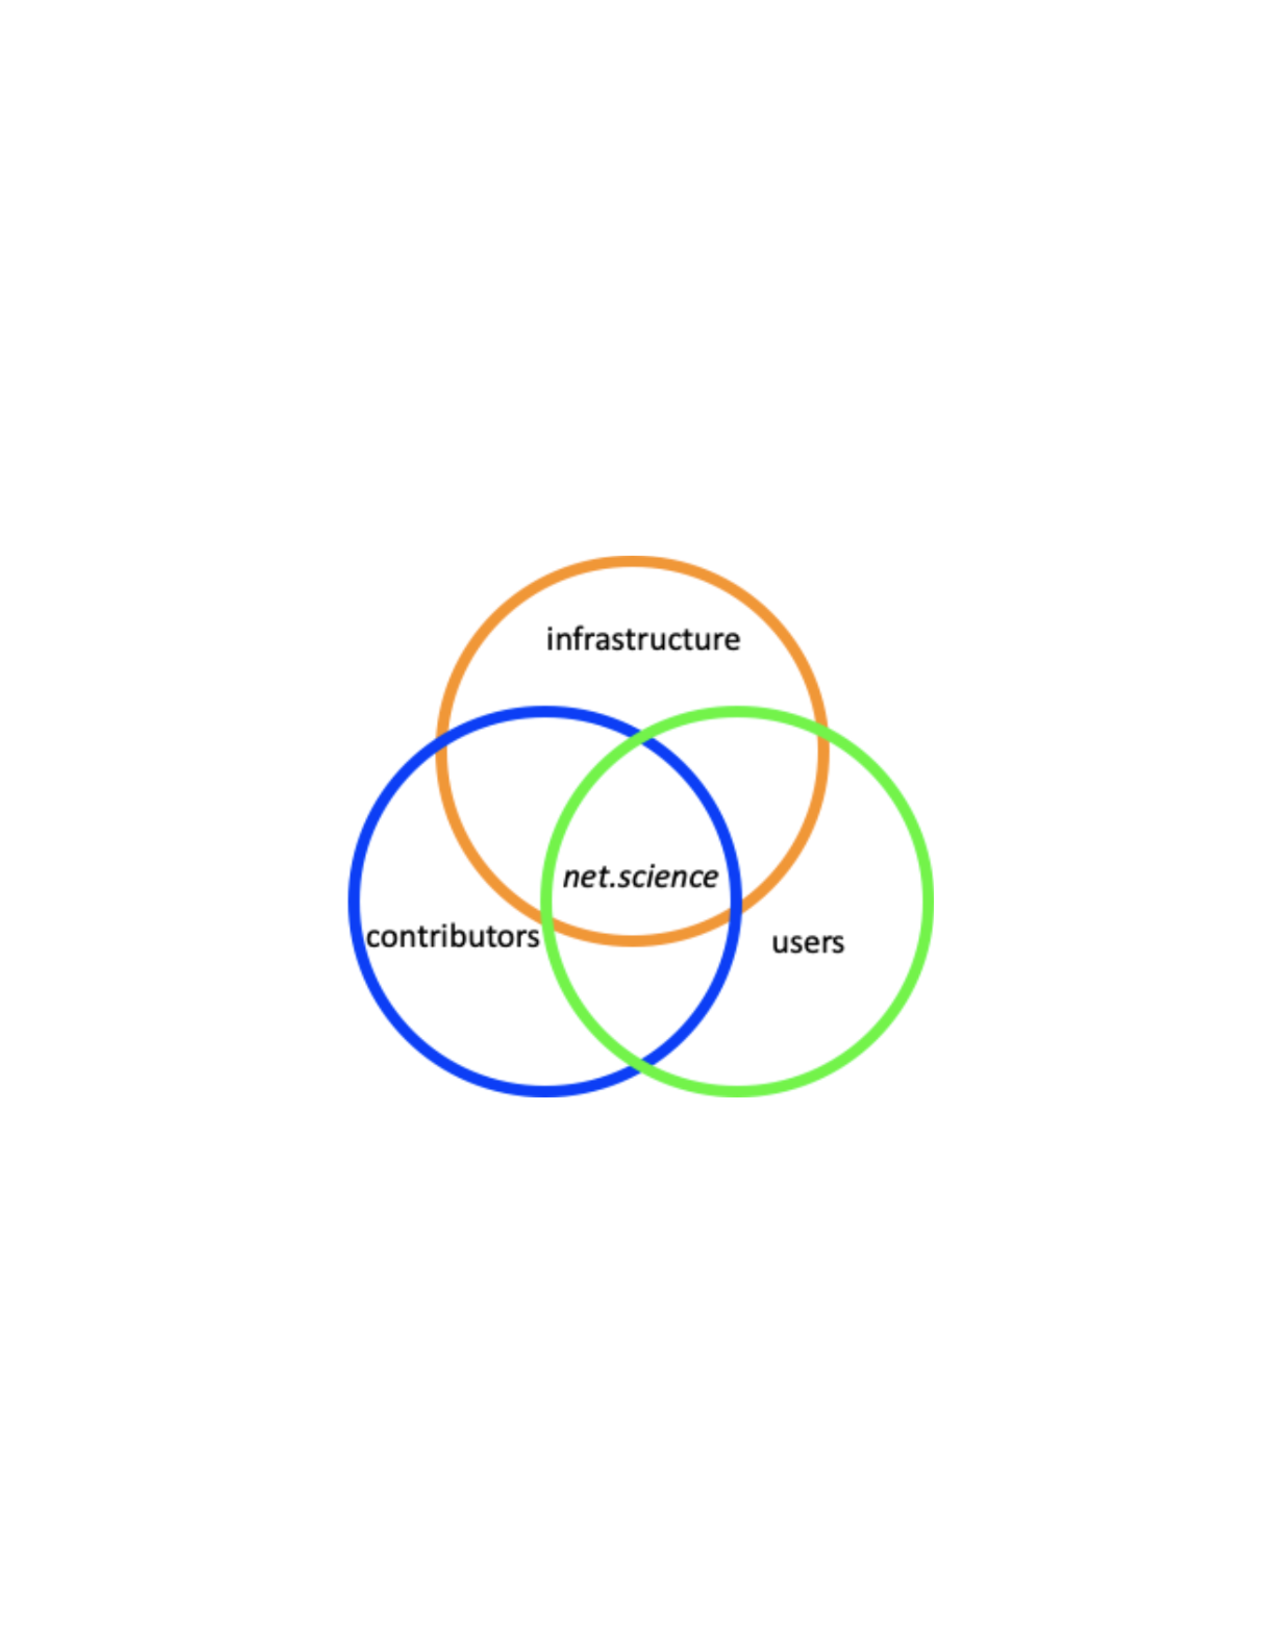
\includegraphics[scale=0.2]{figures/motivation.pdf}
   \end{center}

}
\headerbox{System Description}
          {name=system,column=0,row=1,below=motive}{

\begin{minipage}{.5\textwidth}
\begin{itemize}[leftmargin=*,noitemsep,topsep=0pt]
\item Open access/Open source cyberinfrastructure
\item General purpose network science
\item Community resource
\end{itemize}
\end{minipage}
\hfill
\begin{minipage}{.5\textwidth}
\begin{center}
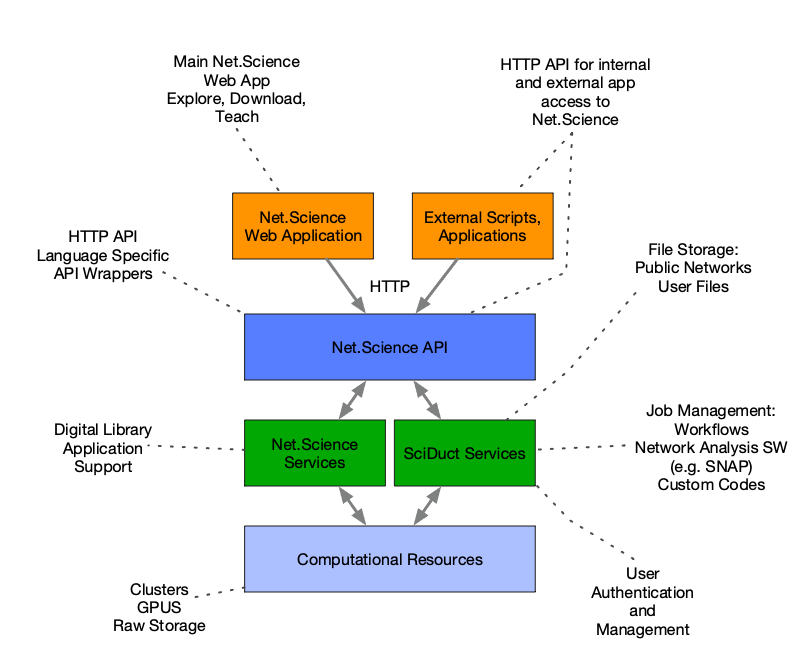
\includegraphics[scale=0.2]{figures/sys_descr.png}
\end{center}
\end{minipage}
}

\headerbox{Networks}
          {name=network,column=0,row=2,below=system}{         

\begin{minipage}{.5\textwidth}        
Labeled Multigraph
\centering
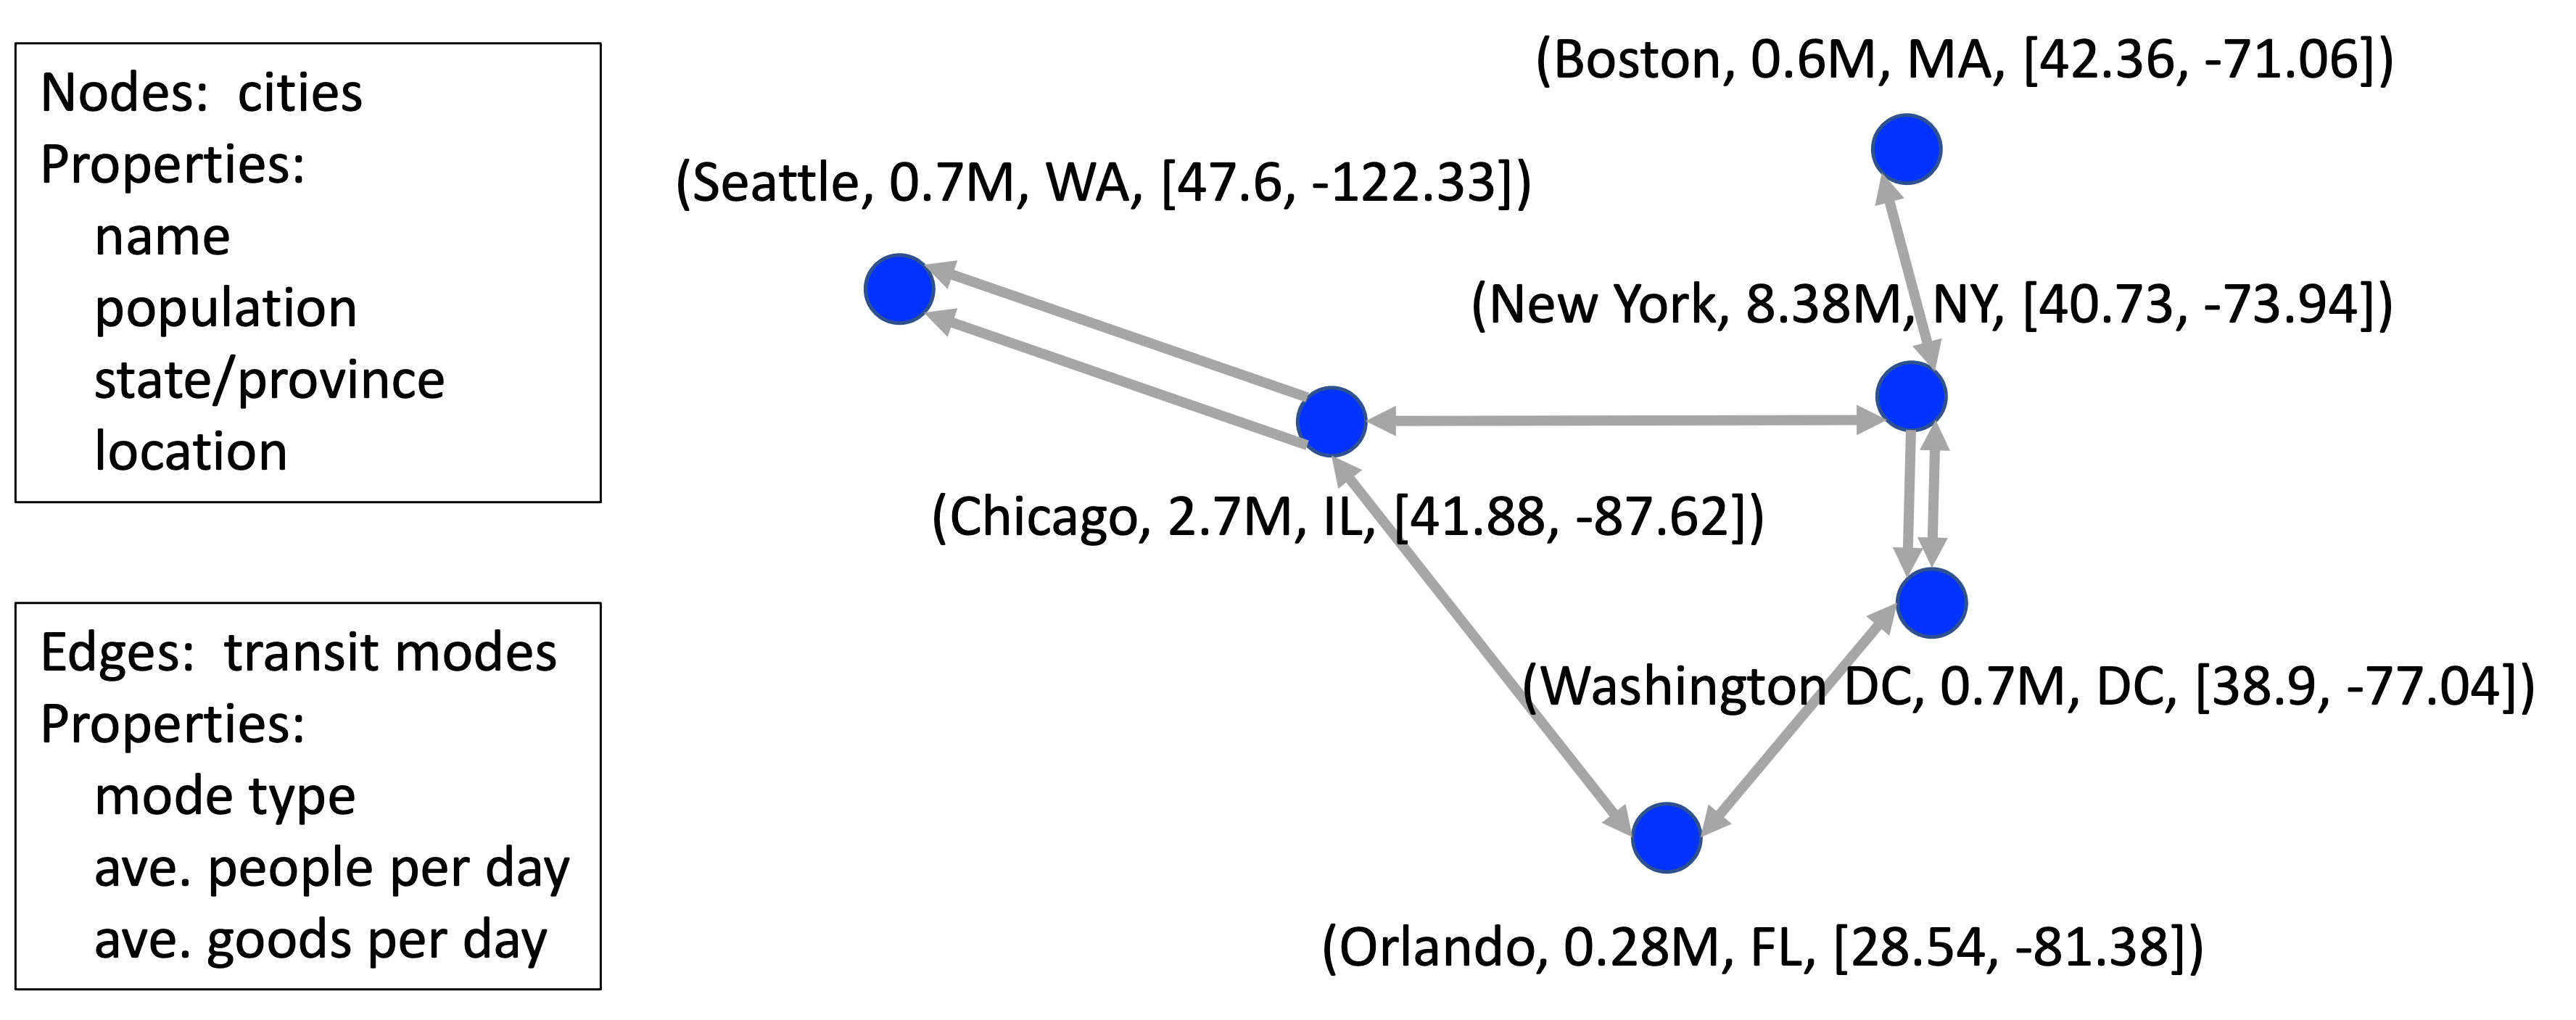
\includegraphics[scale=0.22]{figures/single_net.png}
%\captionof{figure}{Labeled Multigraph\label{label}}
\end{minipage}
\hfill
 \begin{minipage}{.45\textwidth}      
 Multiplex Network
 \centering
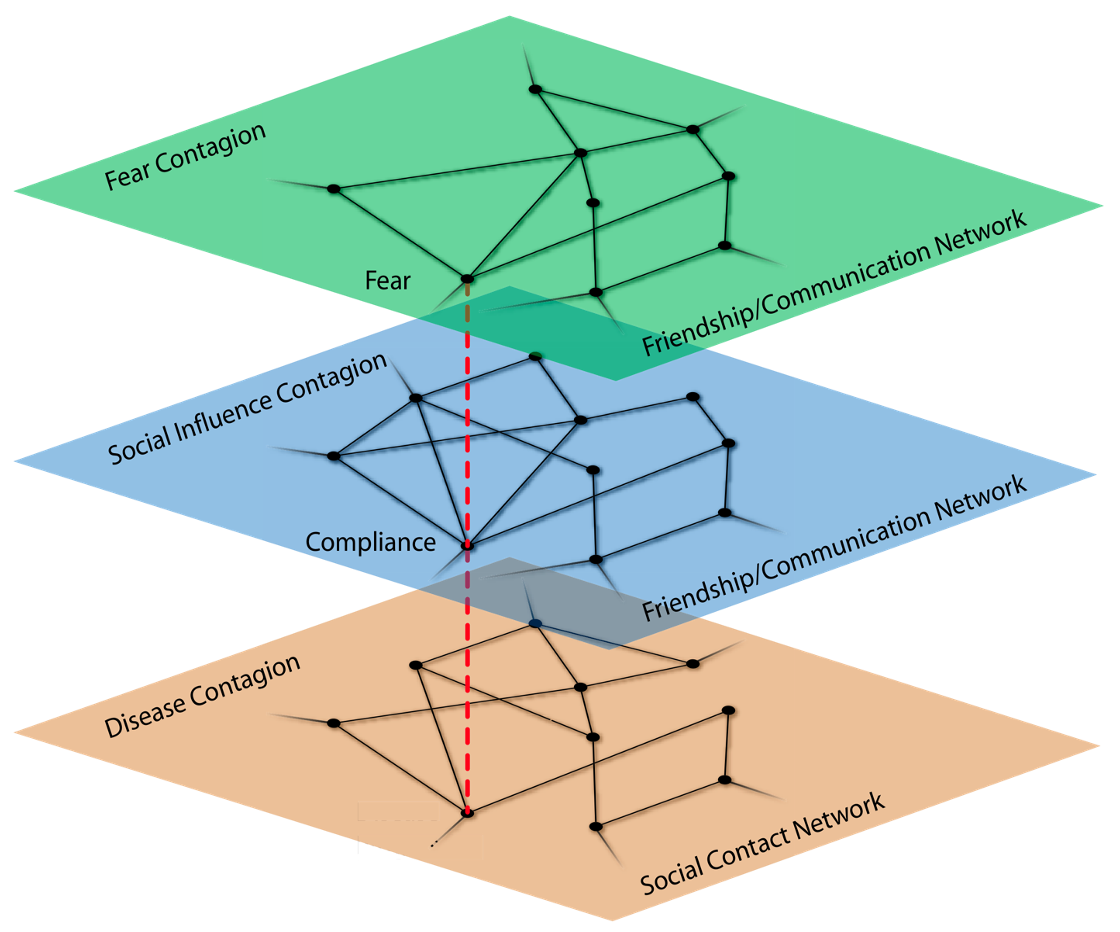
\includegraphics[scale=0.3]{figures/multi_net.png}
%\captionof{figure}{Multiplex Network\label{multiplex}}
\end{minipage}
}
\headerbox{Contributions}
          {name=contri,column=0,row=1 ,below=network}{
\begin{itemize}[leftmargin=*,noitemsep,topsep=0pt]
\item Artifacts
\begin{itemize}
\small{
\item Networks
\item Operations on networks
\item Data collection to generate networks}
\end{itemize}
\item Contributors given full credit in system.
\end{itemize}

}

%%%%%%%%%% Begin Column 1 %%%%%%%%%%

\headerbox{System Views}
          {name=sysViews, column=1,row=0}{
          
\begin{minipage}{.45\textwidth}
\begin{itemize}[leftmargin=*,noitemsep,topsep=0pt]
\item Tasks:  user-supplied, common services, system support
\item Extensible
\end{itemize}
\end{minipage}
\hfill
\begin{minipage}{.55\textwidth}

\begin{center}
Task View
\end{center}

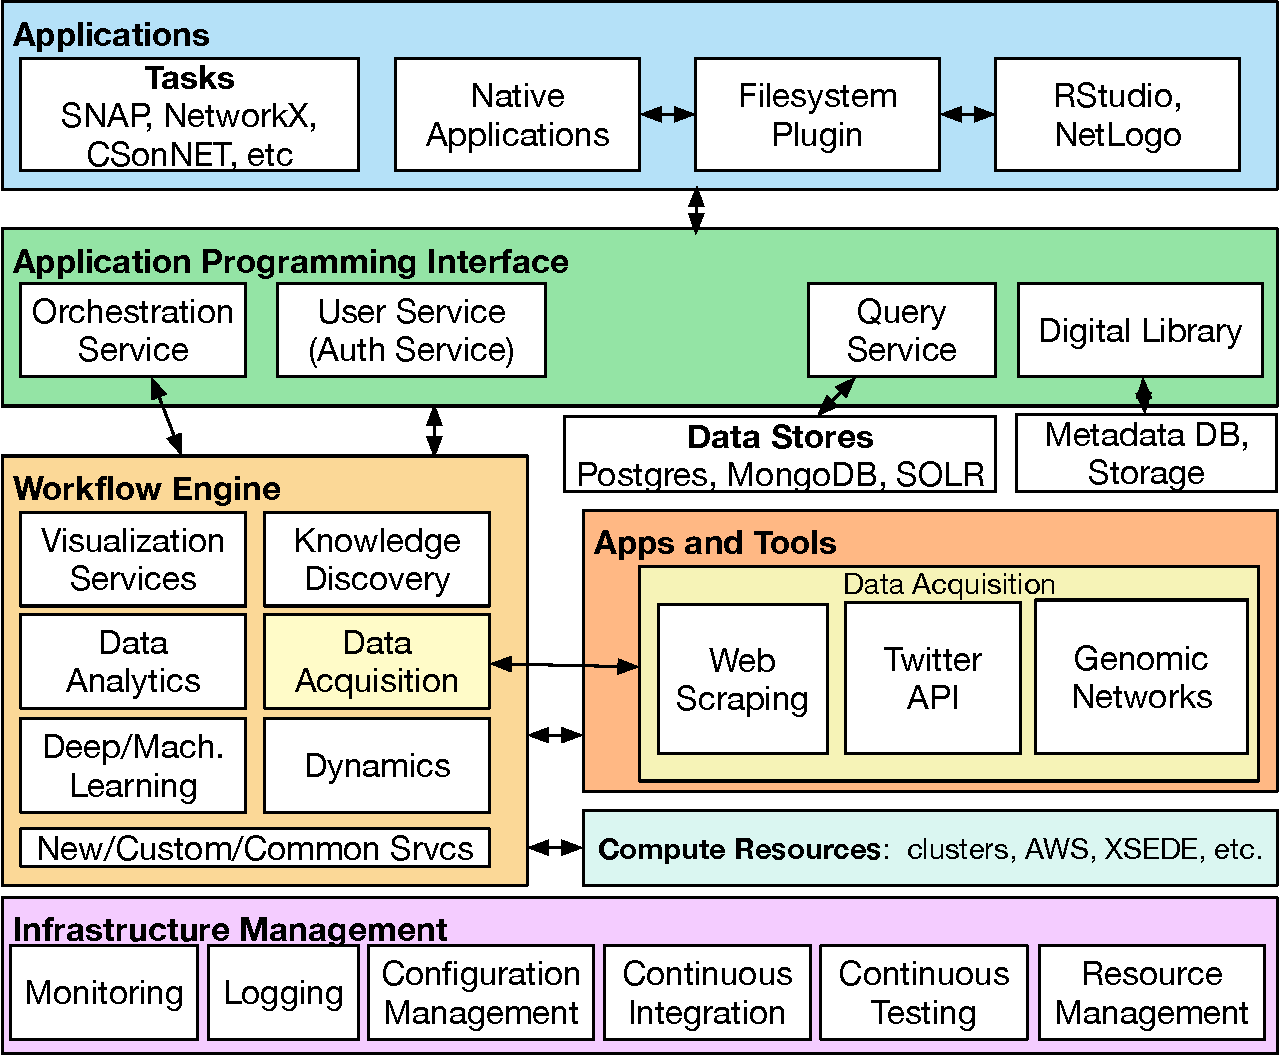
\includegraphics[scale=0.2]{figures/CINSArchV8.pdf} 
\end{minipage}

\begin{minipage}{.29\textwidth}
\begin{itemize}[leftmargin=*,noitemsep,topsep=0pt]
\item Job submission via Web App
\item 3rd party codes use same API
\item Jobs currently run on a cluster
\end{itemize}
\end{minipage}
\hfill
\begin{minipage}{.71\textwidth}
\vspace{5mm}
\begin{center}
Process View
\end{center}
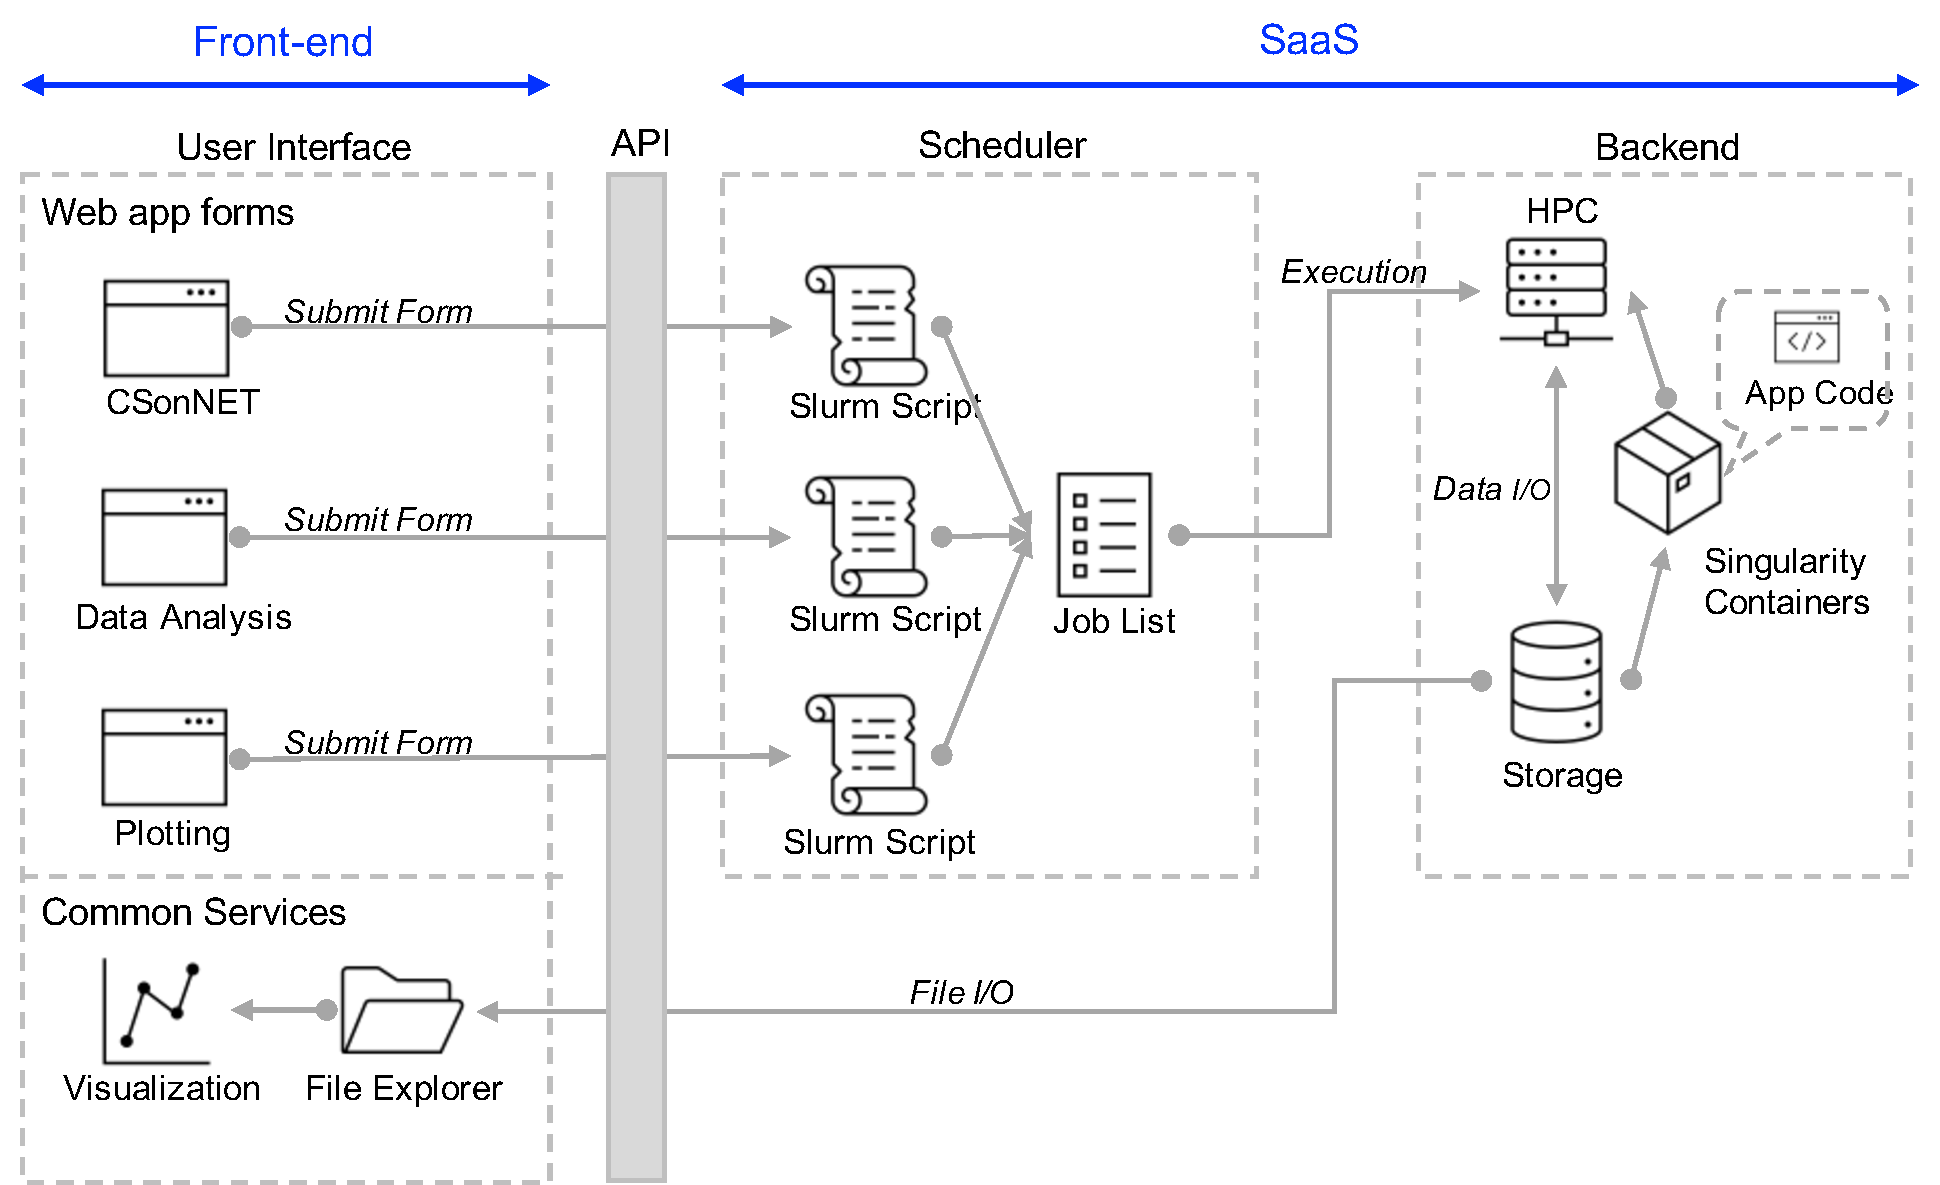
\includegraphics[scale=0.2]{figures/netsci_ops_v6.pdf}
\end{minipage}

}

\headerbox{SciDuct}
          {name=sciduct,column=1,row=1,below=sysViews}{
          
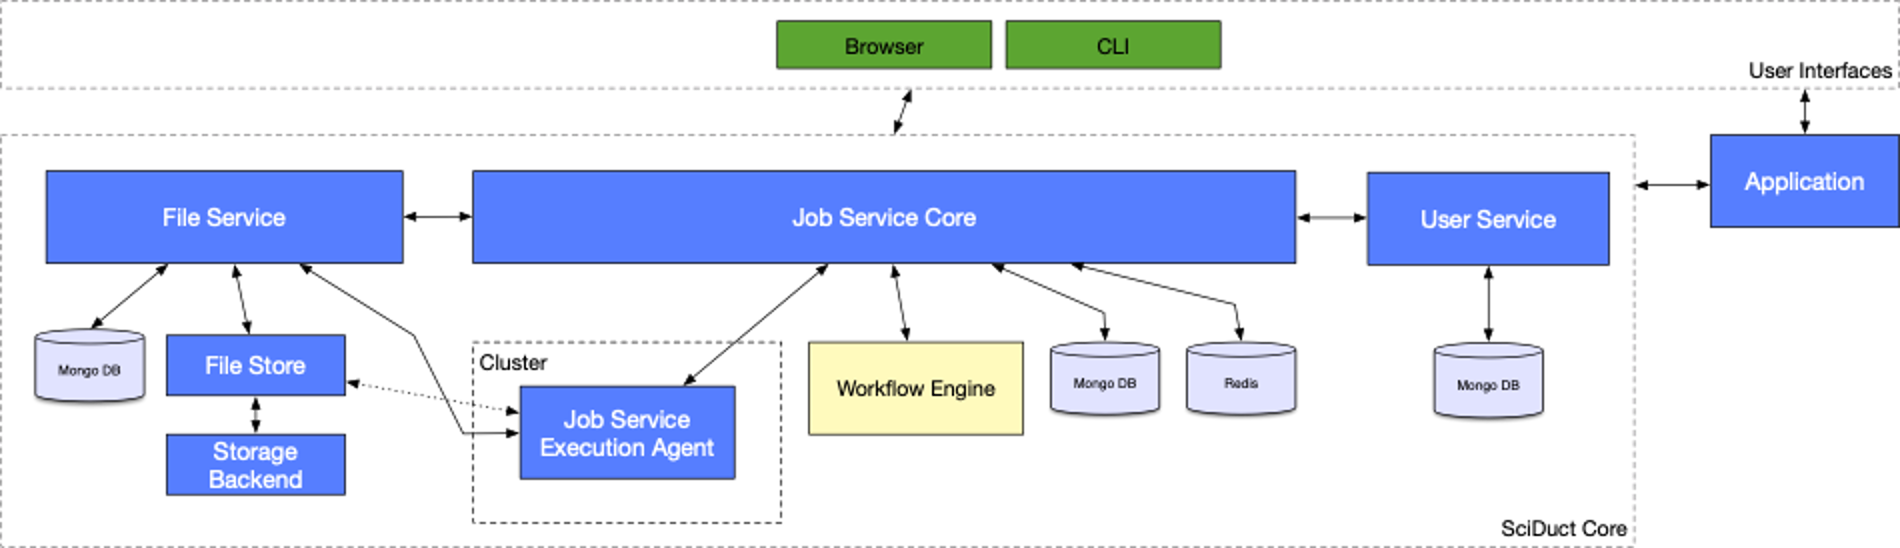
\includegraphics[scale=0.27]{figures/sciduct.png}

\vspace{5mm}
\noindent 
\begin{minipage}[t]{0.32\columnwidth}
User Service

\small{\begin{itemize}[leftmargin=*,noitemsep,topsep=0pt]
	\item Authentication
	\item Teams
	\item Preferences
\end{itemize}}
\end{minipage}
\hfill
\noindent
\begin{minipage}[t]{0.32\columnwidth}
File Service

\small{\begin{itemize}[leftmargin=*,noitemsep,topsep=0pt]
	\item Data stores
	\item File validations
	\item Query system
\end{itemize}}

\end{minipage}
\hfill
\noindent
\begin{minipage}[t]{0.32\columnwidth}
Job Service
\small{\begin{itemize}[leftmargin=*,noitemsep,topsep=0pt]
	\item Task Executor
	\item Manages workspaces
	\item Container-based 

\end{itemize}}

\end{minipage}
}


\headerbox{Containerization}
          {name=contain,column=1,row=2,below=sciduct}{
          
% 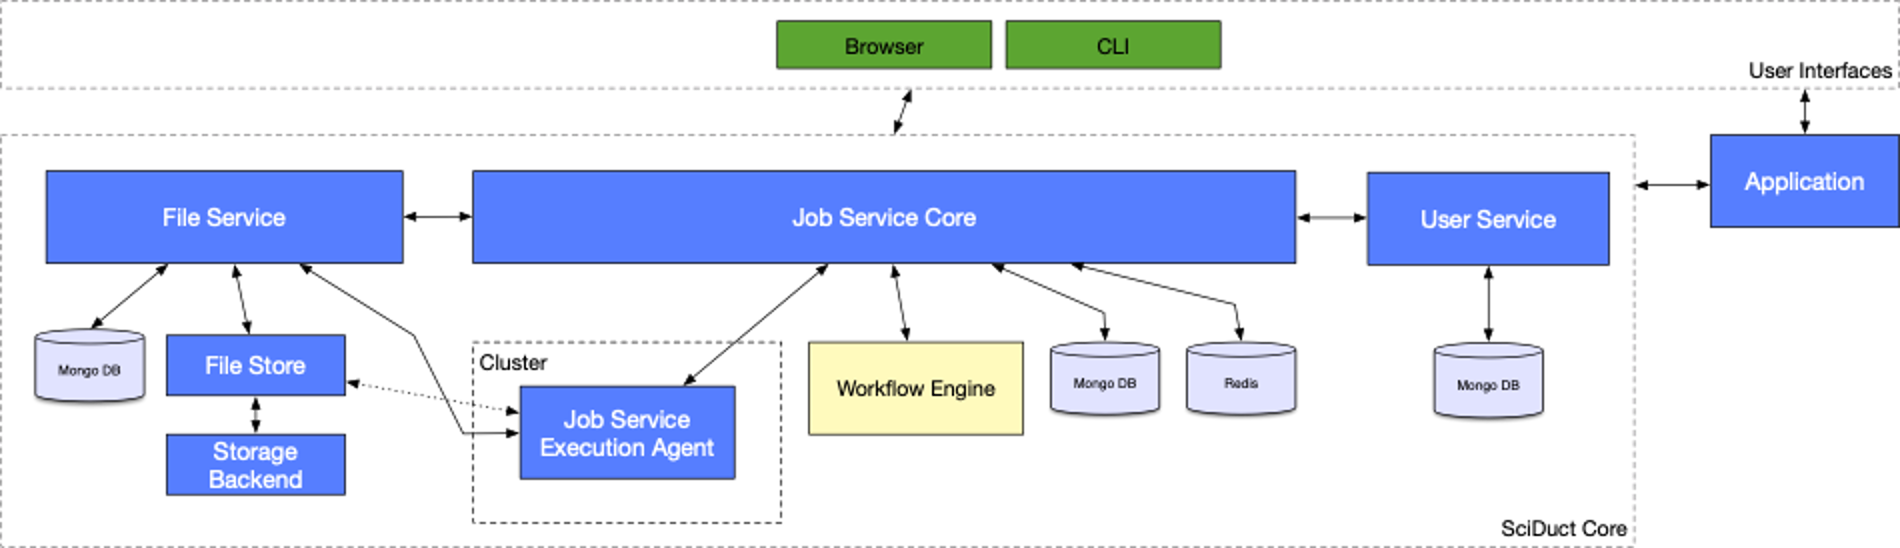
\includegraphics[scale=0.3]{figures/sciduct.png}
something on containerization
} 

%%%%%%%%%% Begin Column 2 %%%%%%%%%%

\headerbox{Front End Interface}
          {name=frontend,column=2,row=0}{
          

\begin{minipage}{.29\textwidth}
\begin{itemize}[leftmargin=*,noitemsep,topsep=0pt]
\item Main screen, contagion simulation
\item Discrete time, propagation on networks
\end{itemize}
\end{minipage}
\hfill
\begin{minipage}{.71\textwidth}         
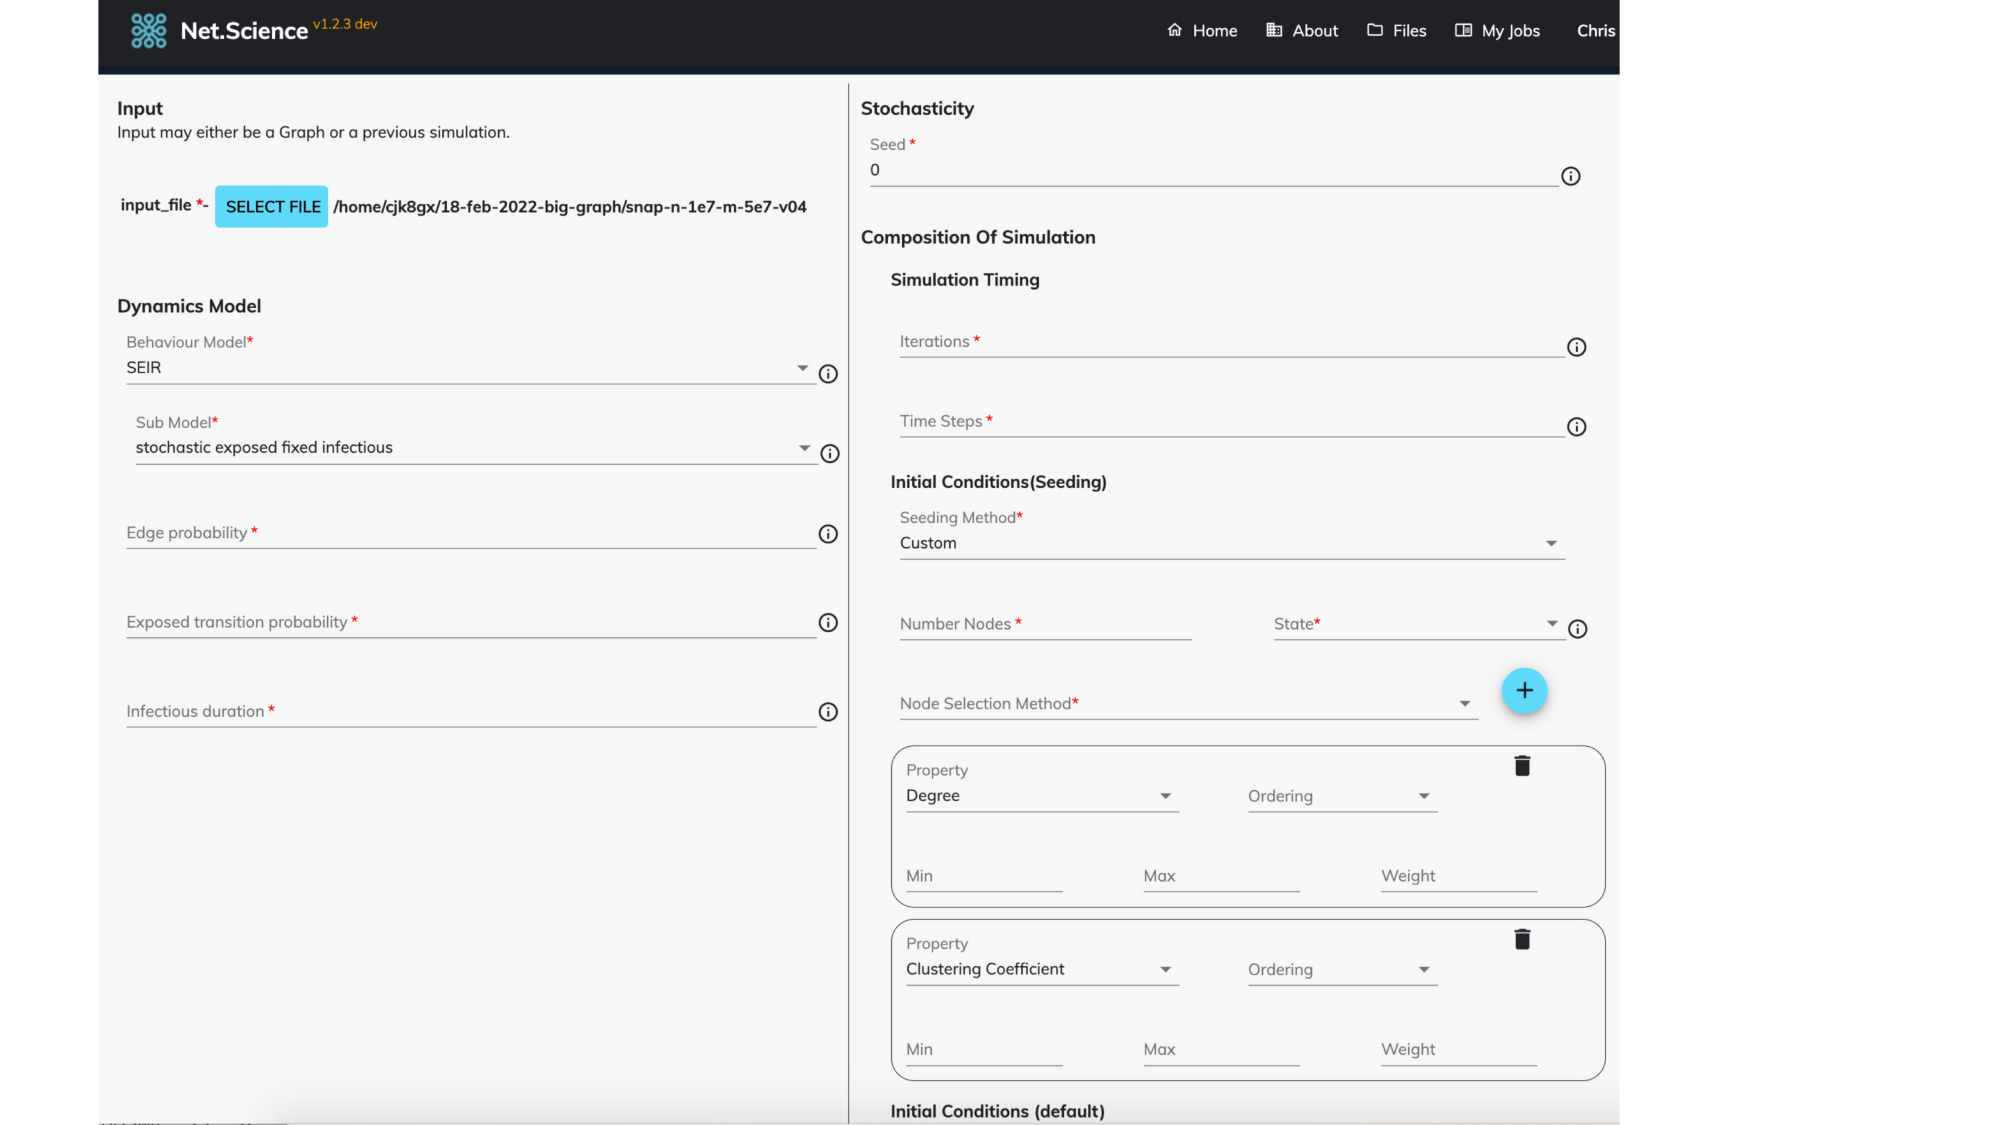
\includegraphics[scale=0.25]{figures/csonnet-model-seeds.pdf} 
\end{minipage}
\begin{minipage}{.29\textwidth}
\begin{itemize}[leftmargin=*,noitemsep,topsep=0pt]
\item Main screen, plot generation
\item Publication quality, contagion results
\end{itemize}
\end{minipage}
\hfill
\begin{minipage}{.71\textwidth}  
\vspace{5mm}
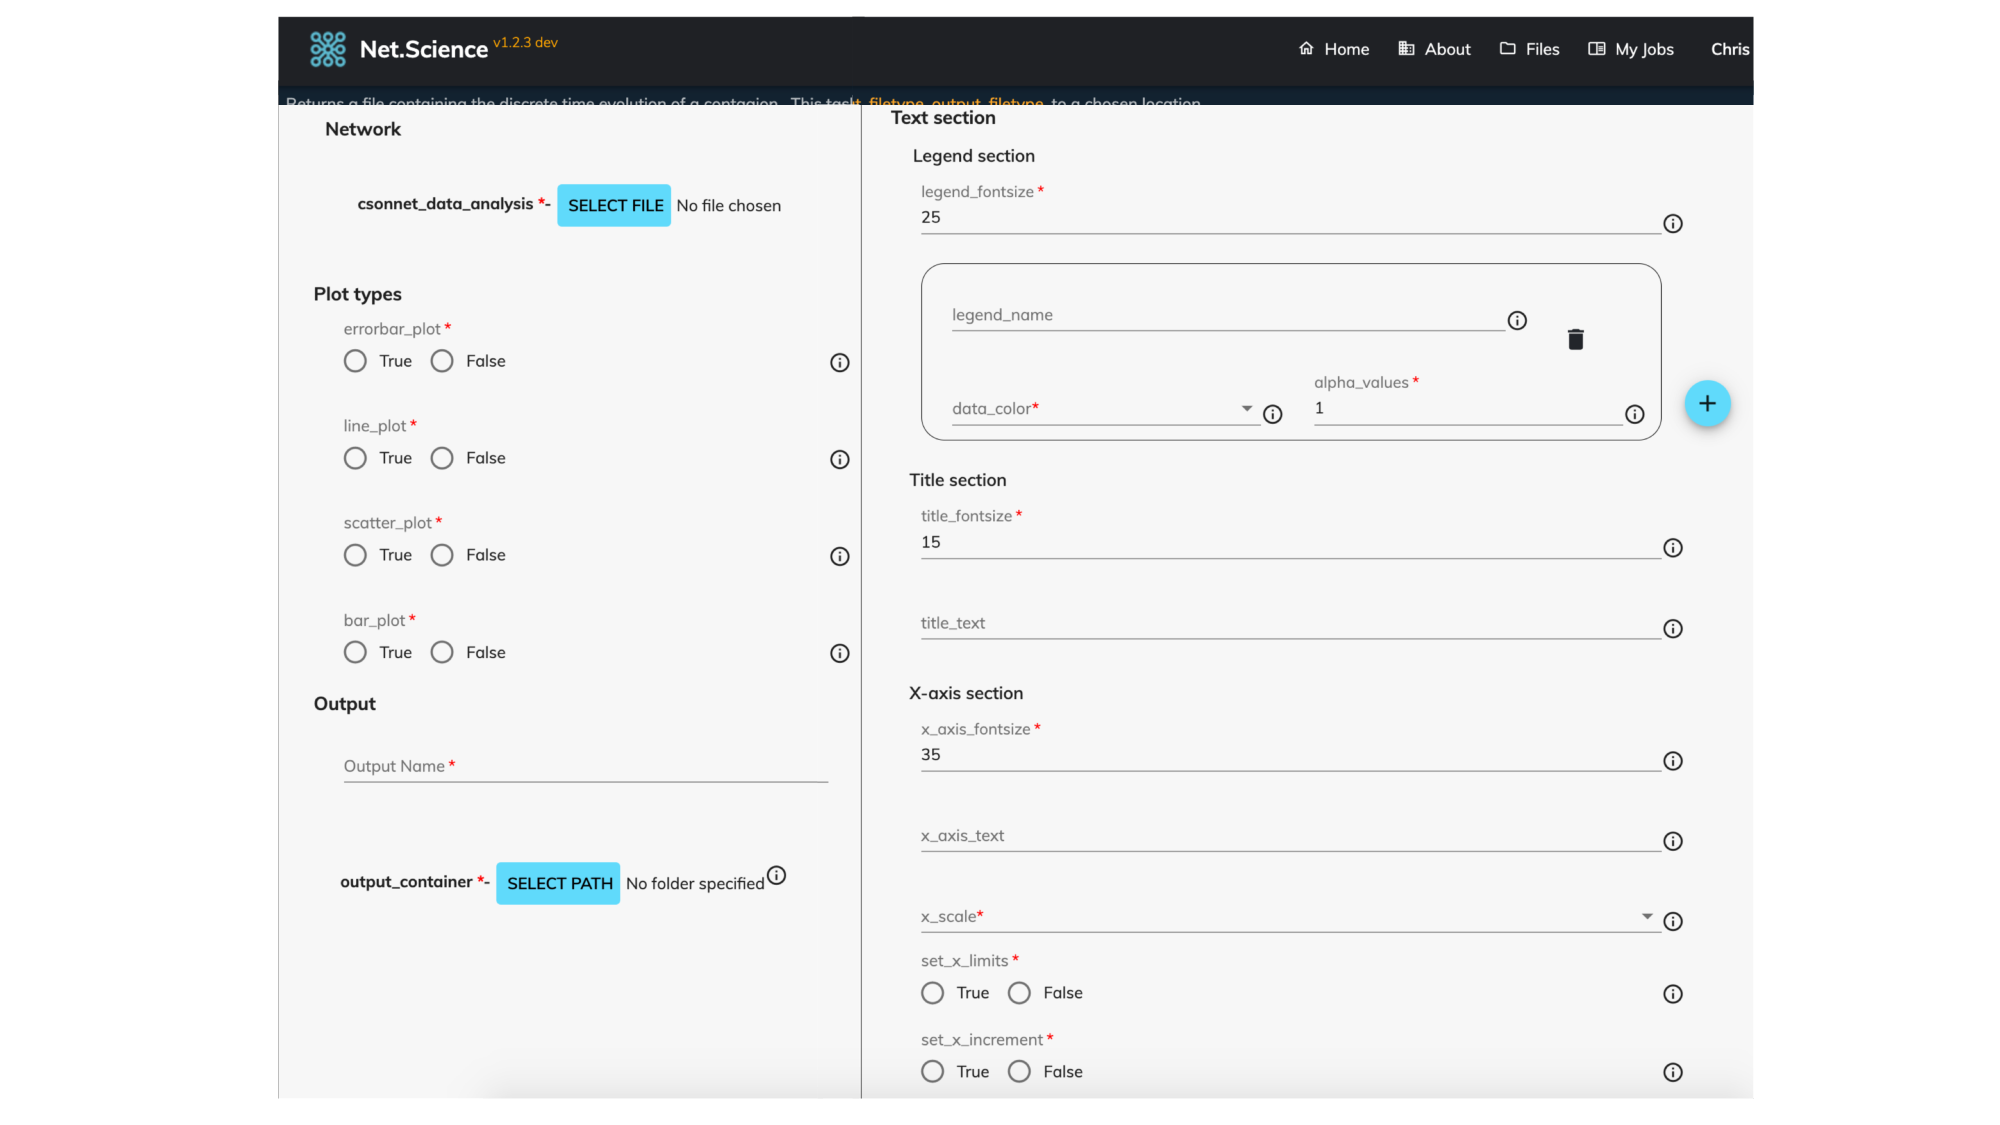
\includegraphics[scale=0.26]{figures/plot_input.pdf}
\end{minipage}
\hfill
\vspace{5mm}

\begin{minipage}{0.48\linewidth}
Graph:  nodes and edge are those of graph

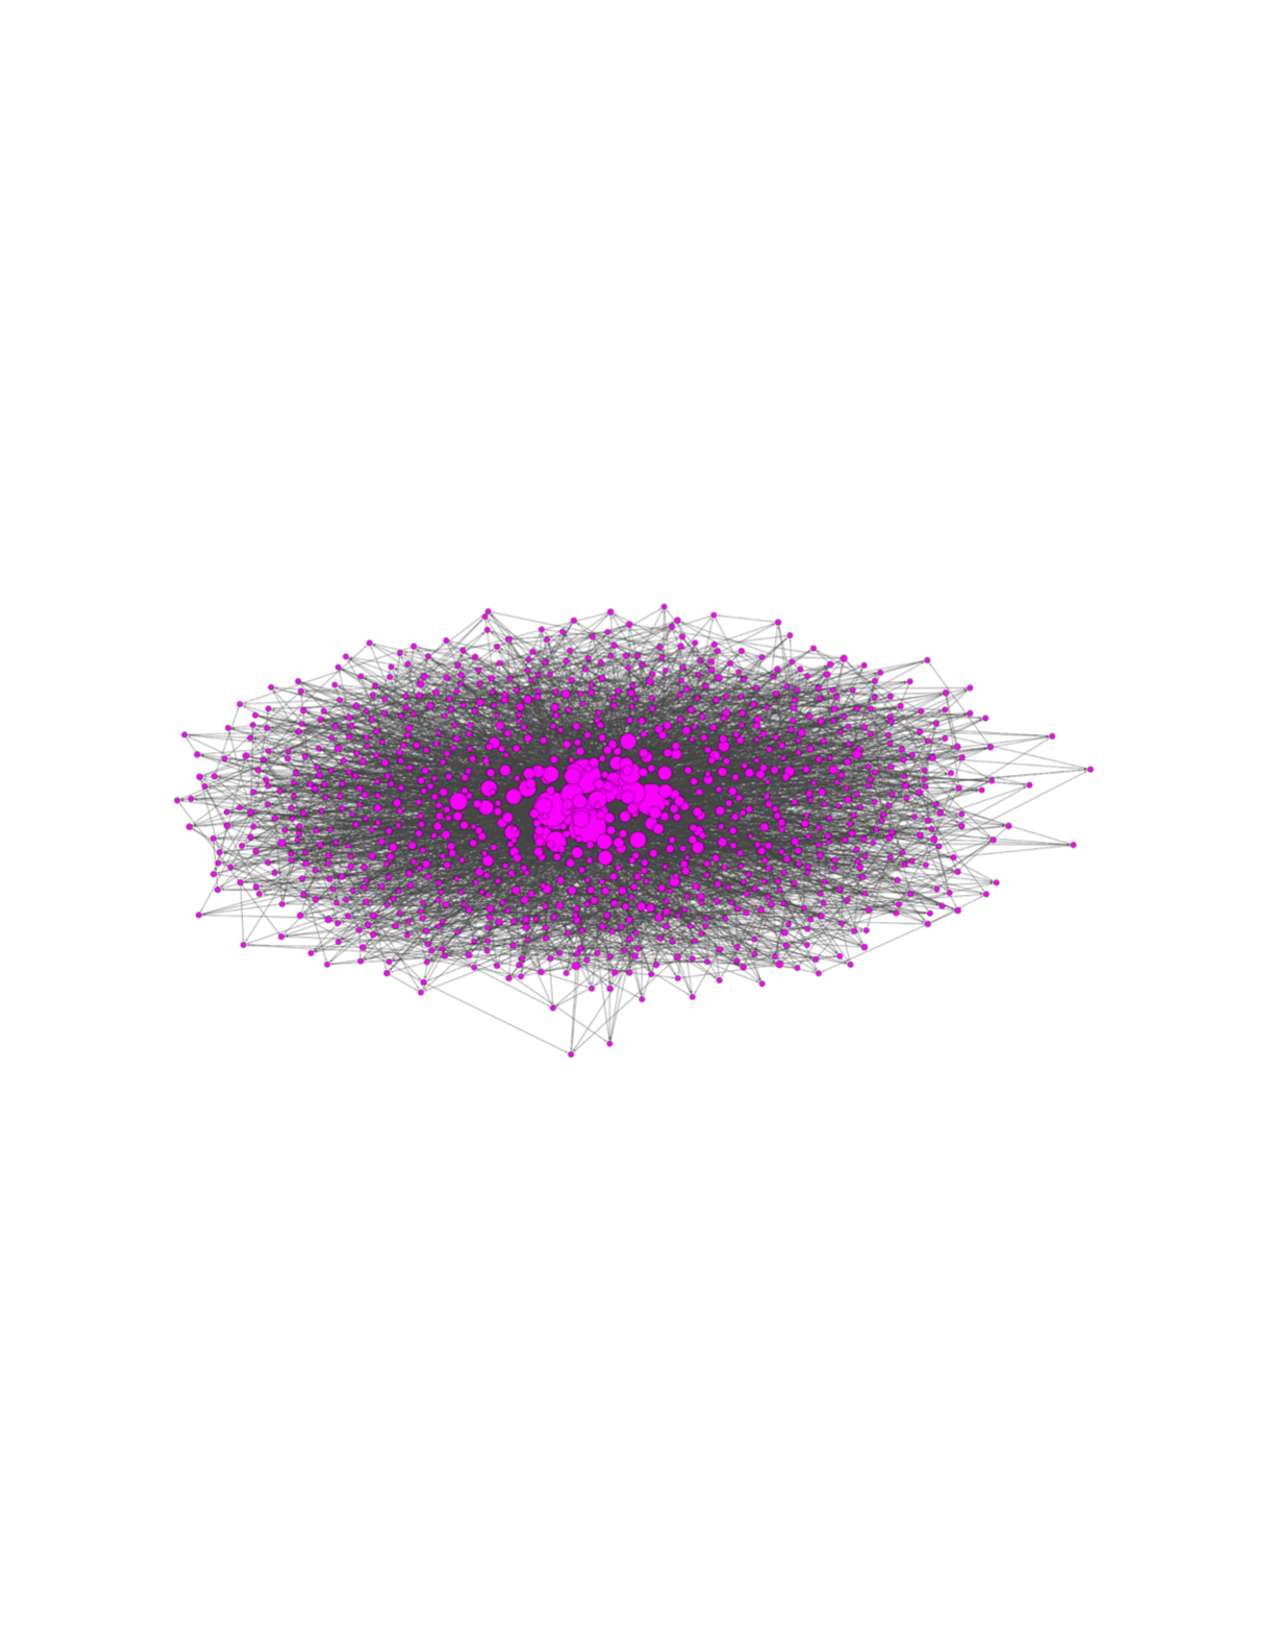
\includegraphics[scale=0.3]{figures/graph_nodes.pdf} 
\end{minipage}
\hfill
\begin{minipage}{0.48\linewidth}

Graph:  nodes are communities
and edge are those of between communities

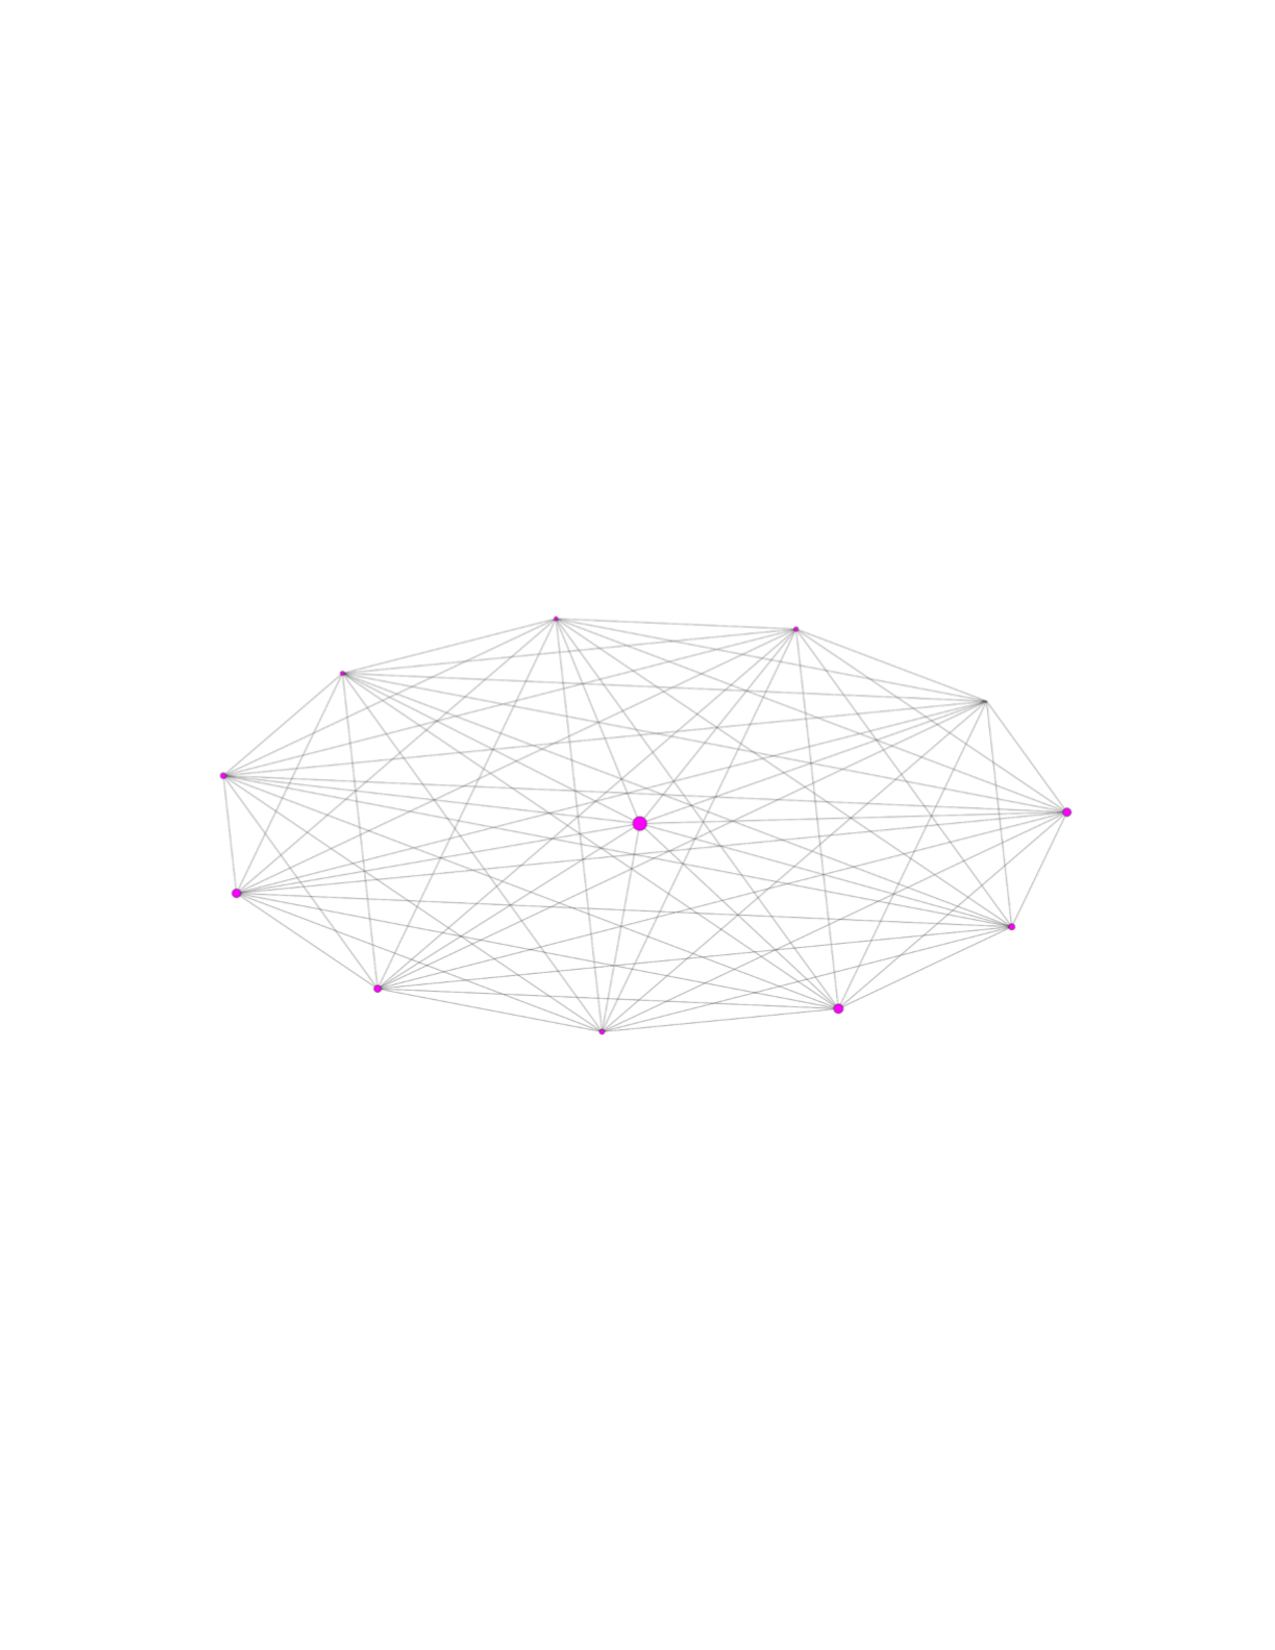
\includegraphics[scale=0.3]{figures/graph_community.pdf} 
\end{minipage}

\vspace{5mm}
pngraph visualization

\begin{center}
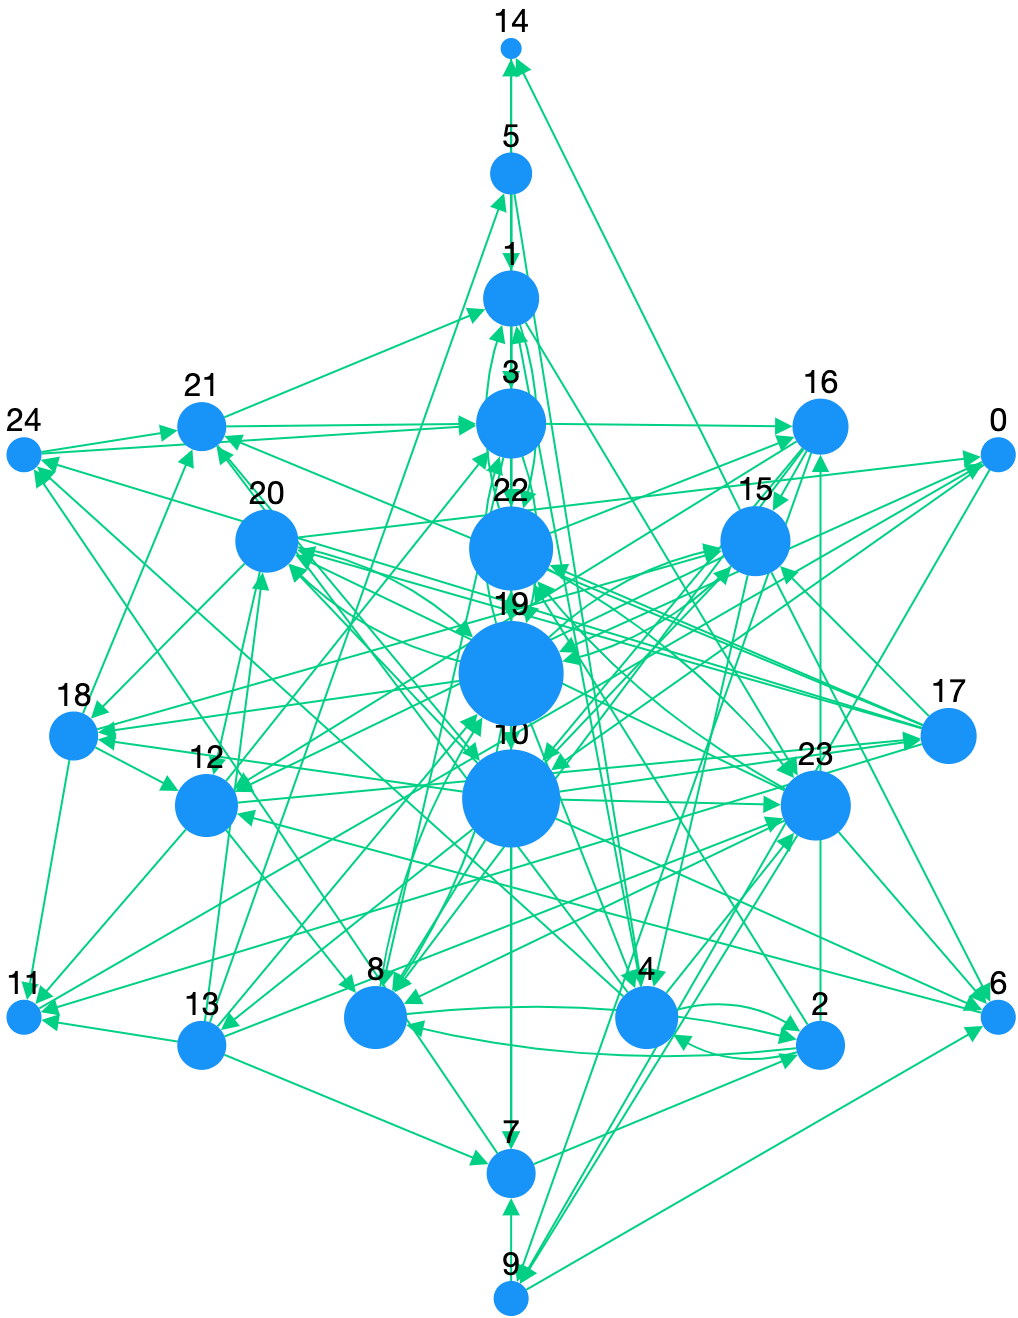
\includegraphics[scale=0.12]{figures/gnm-25-100_pngraph.png} 
\end{center}
}

\headerbox{Computational Tasks}
          {name=tasks,column=3,row=0}{


\begin{itemize}[leftmargin=*,noitemsep,topsep=0pt]
\item User Applications:  Example CSonNet
\end{itemize}

\begin{minipage}{0.5\linewidth}
\centering
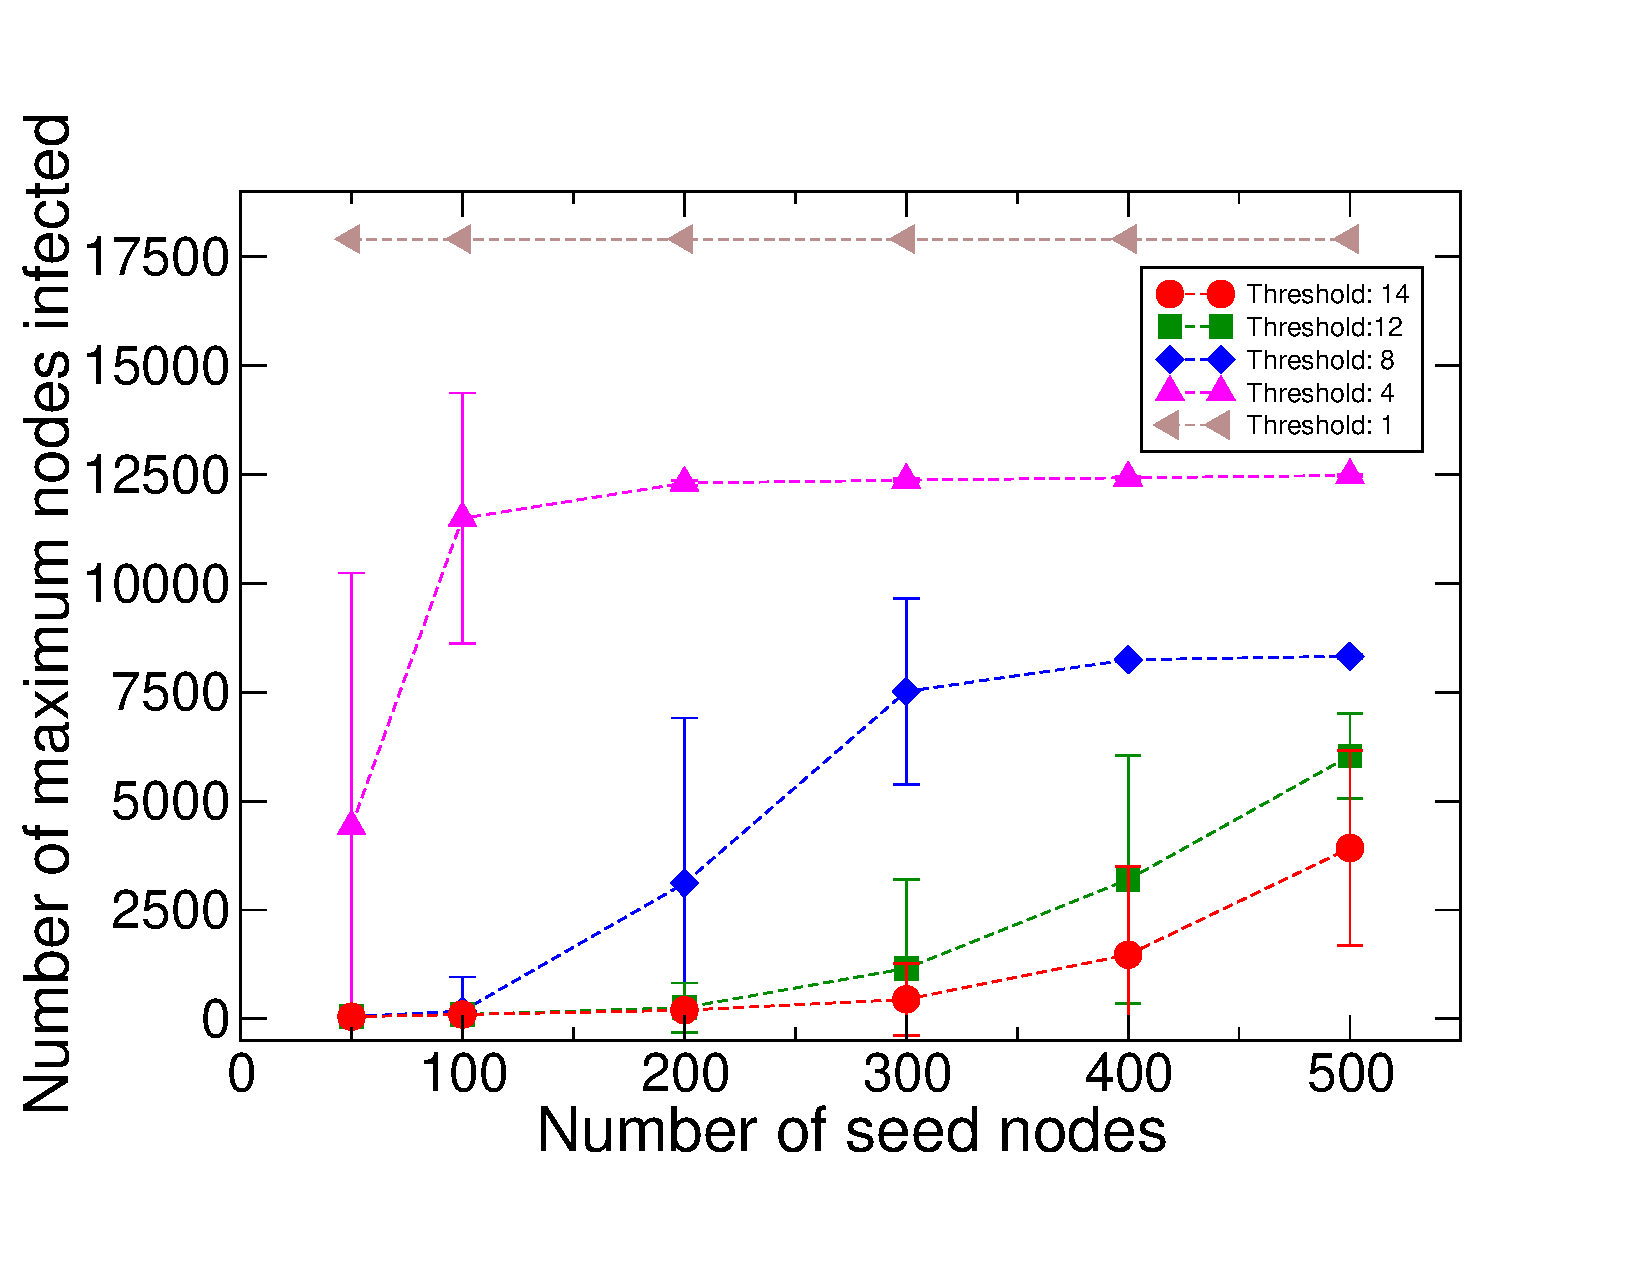
\includegraphics[scale=0.16]{figures/astroph_threshold_cs.pdf} 
\end{minipage}
\hfill
\begin{minipage}{0.5\linewidth}
\centering
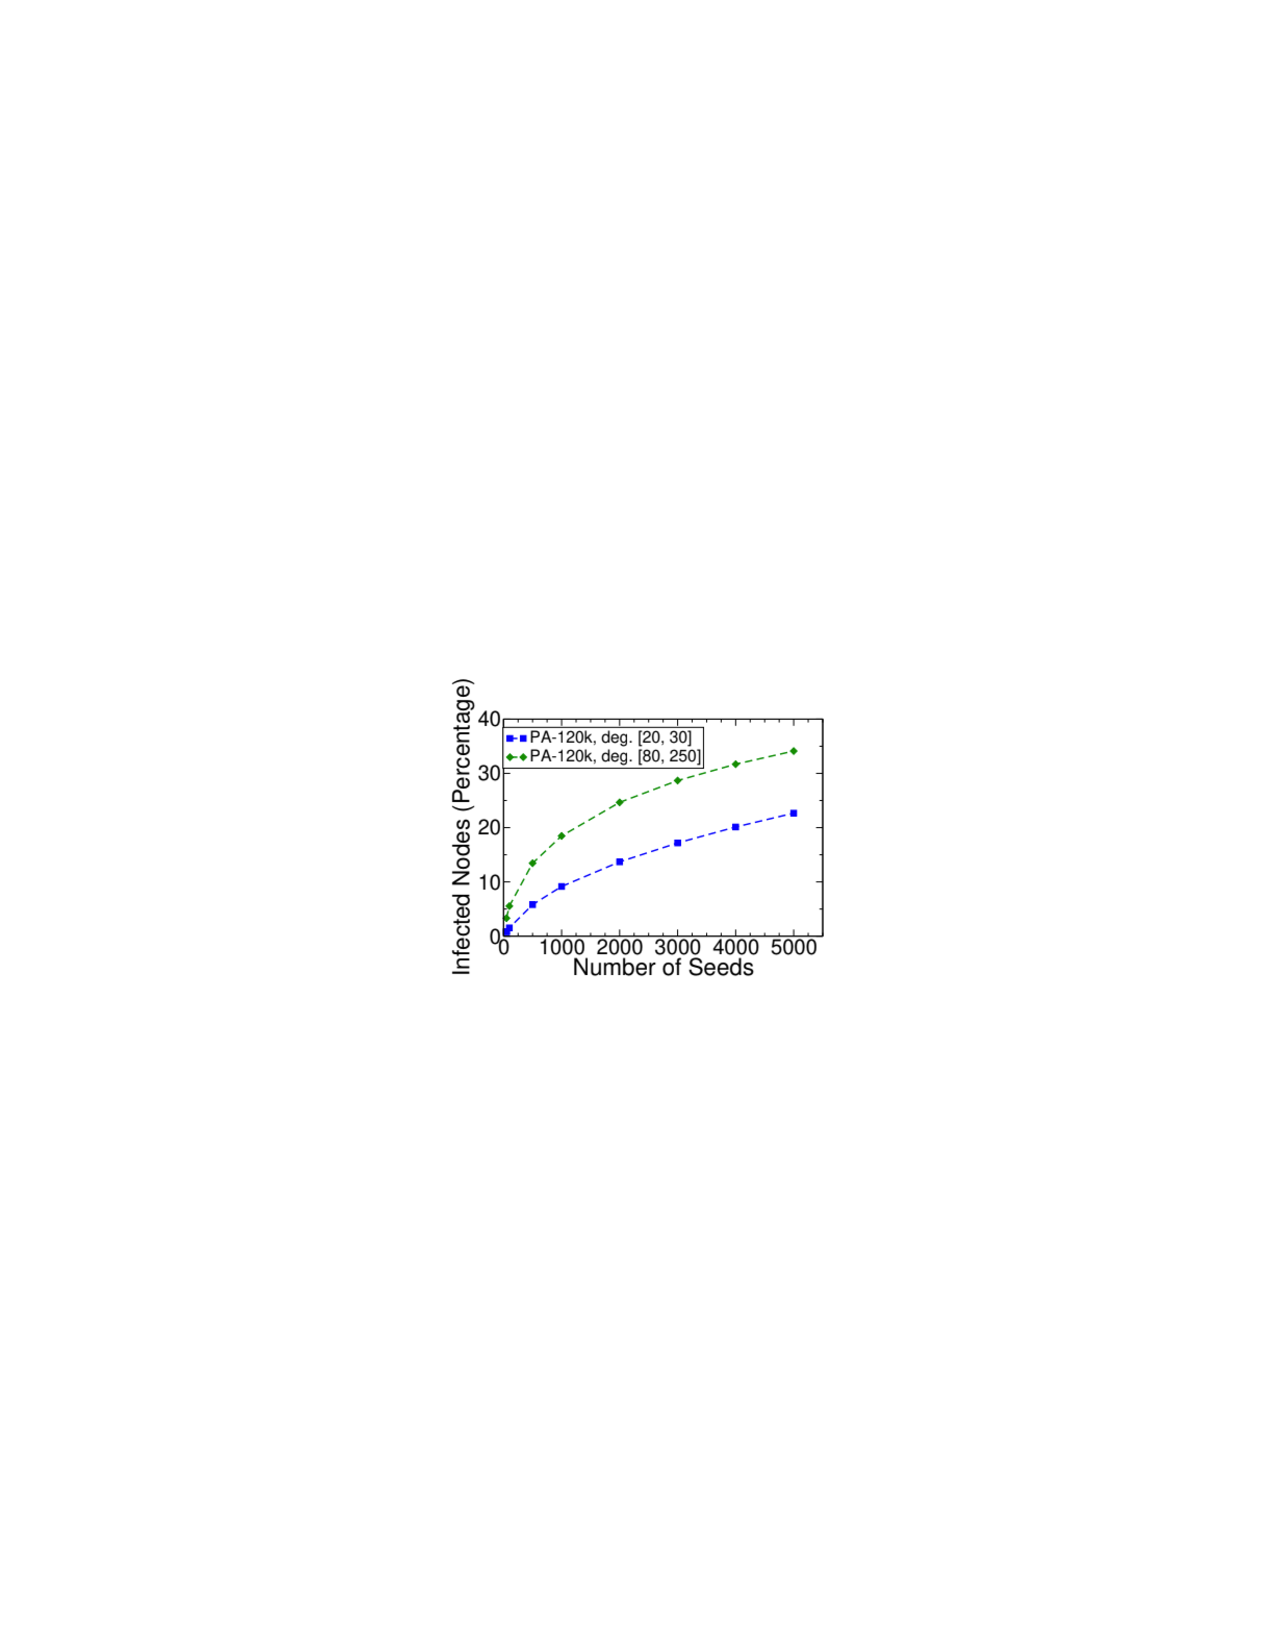
\includegraphics[scale=0.6]{figures/clustering_seed.pdf} 
\end{minipage}
\hfill
\begin{minipage}{0.5\linewidth}
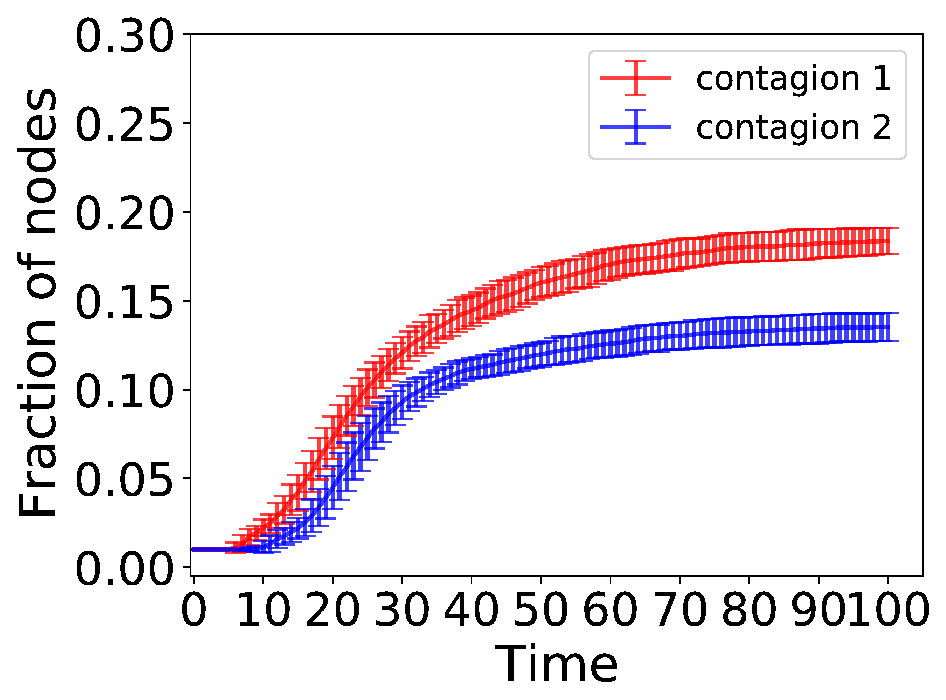
\includegraphics[scale=0.27]{figures/danville_asym_interaction_100ns_fraction_cum_errorbar.eps} 
\end{minipage}
\vspace{5mm}
\hfill
\begin{minipage}{0.48\linewidth}
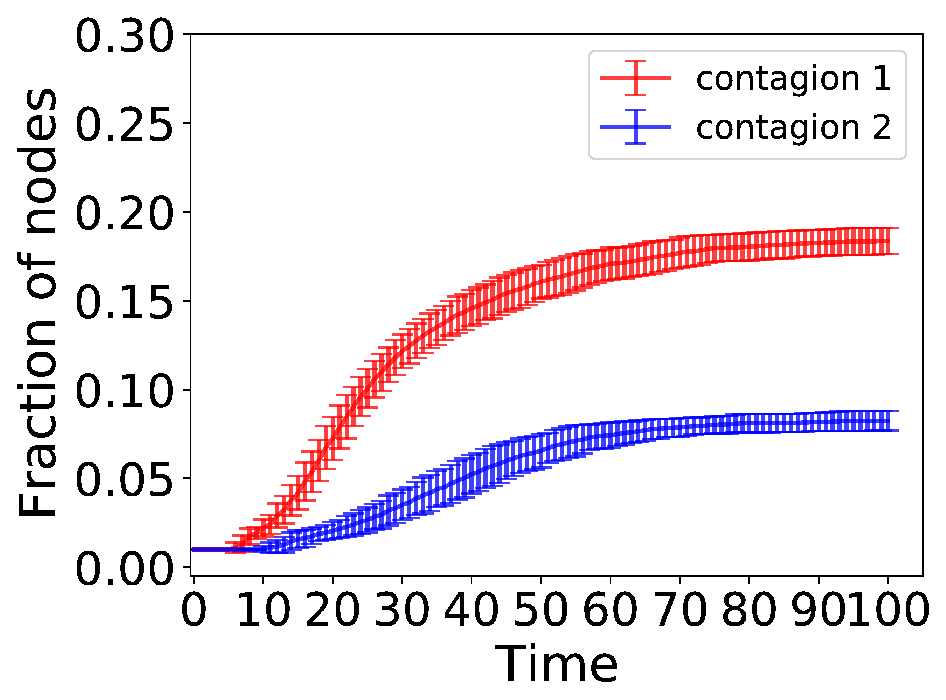
\includegraphics[scale=0.27]{figures/danville_no_interaction_100ns_fraction_cum_errorbar.eps} 
\end{minipage}
%	\begin{itemize}
%	\item CSONNET (Graph Seeding, Plotting)
%	\item Structural Analysis
%	\item Graph Generation
%	\end{itemize}
\begin{itemize}[leftmargin=*,noitemsep,topsep=0pt]
\item Common Services:  Example Graph Transformations
\end{itemize} 
\hfill
\begin{minipage}{0.45\linewidth}
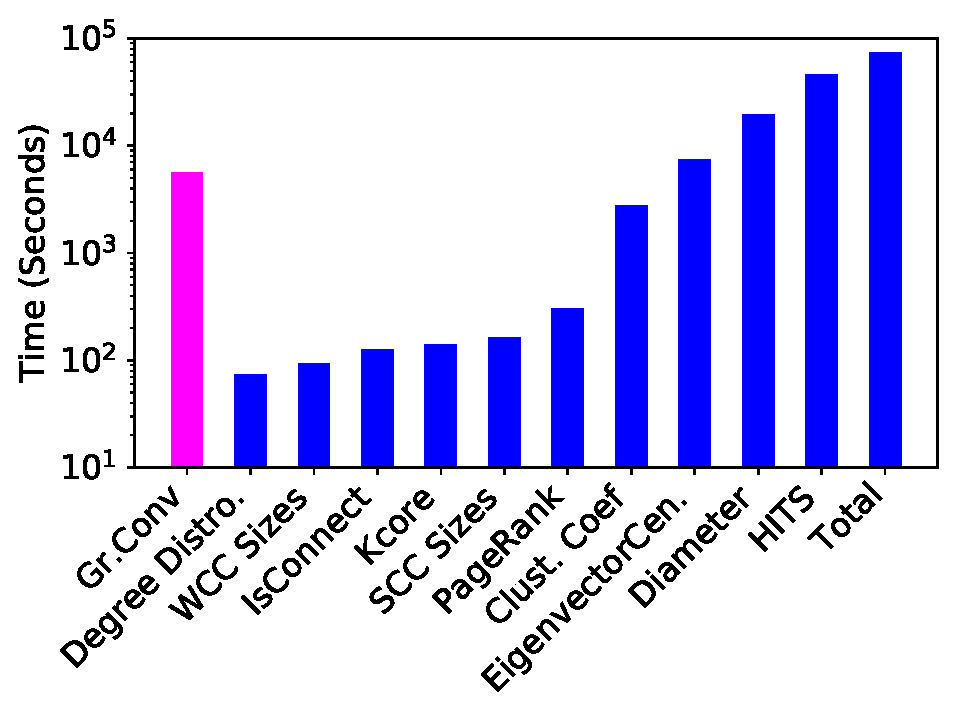
\includegraphics[scale=0.27]{figures/g4_timing.pdf} 
\end{minipage}
\hfill
\begin{minipage}{0.45\linewidth}
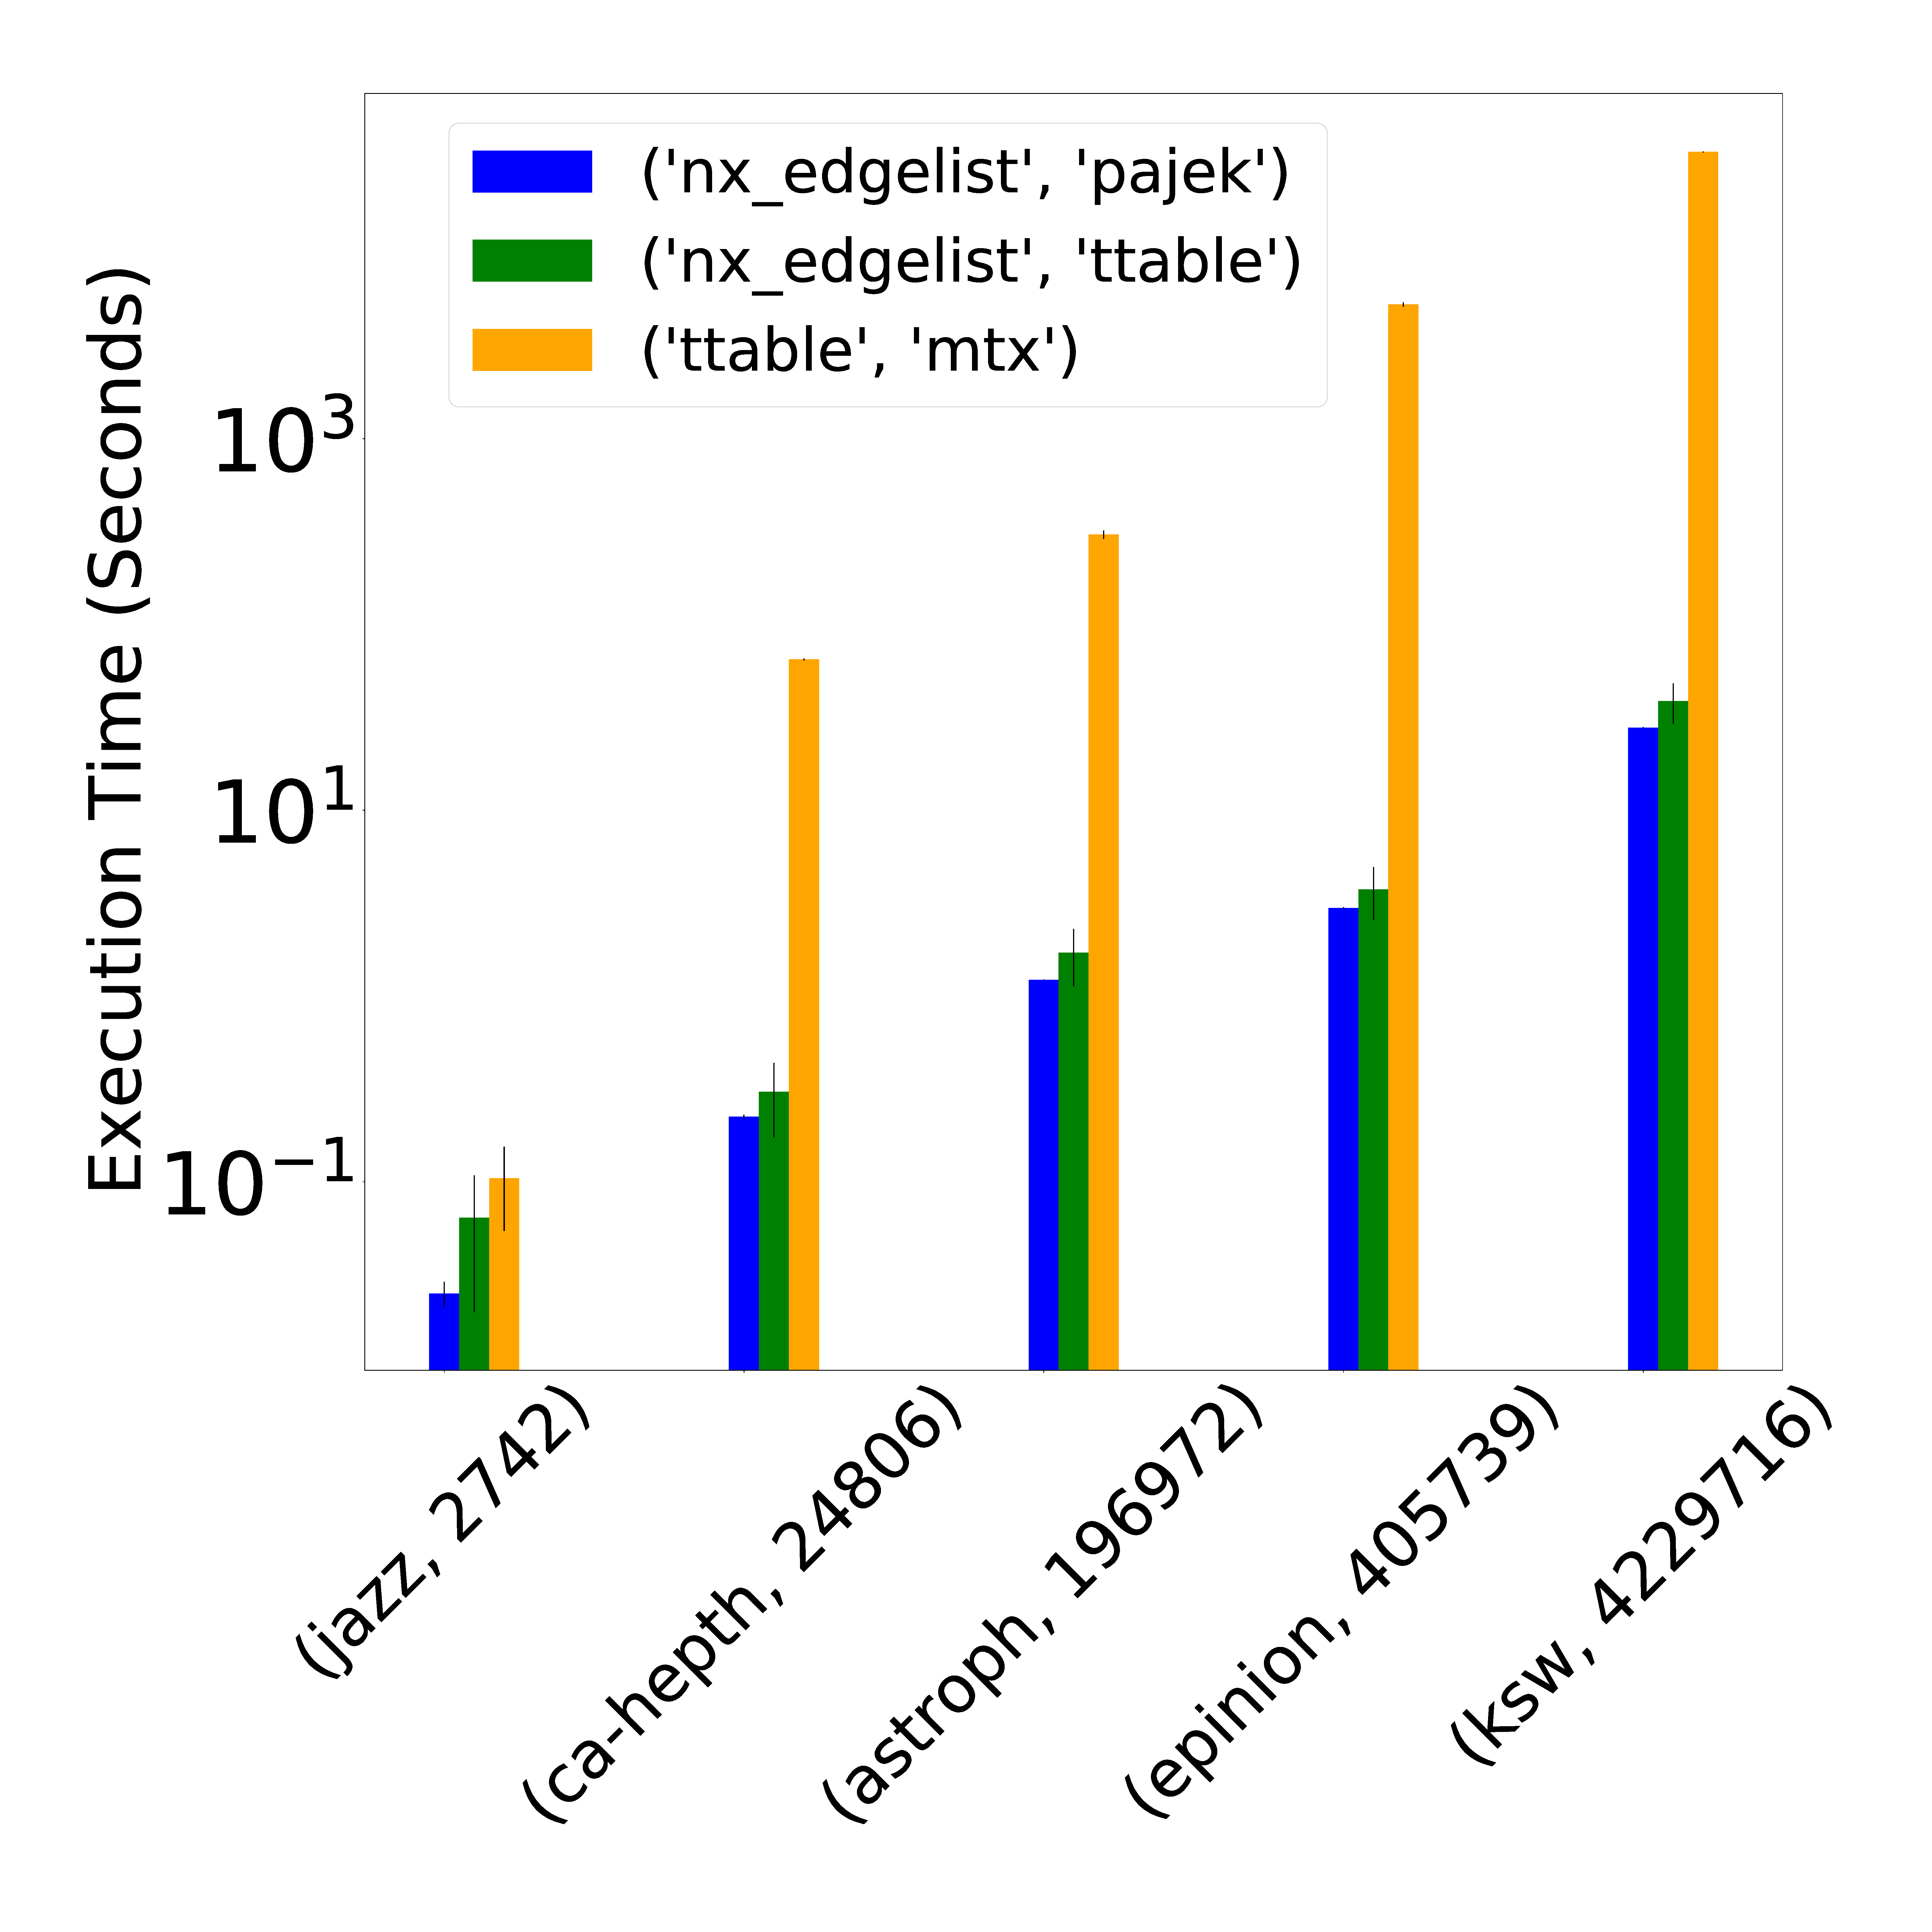
\includegraphics[scale=0.038]{figures/scatter_bar_to_ttable.pdf}
\end{minipage}
\begin{center}
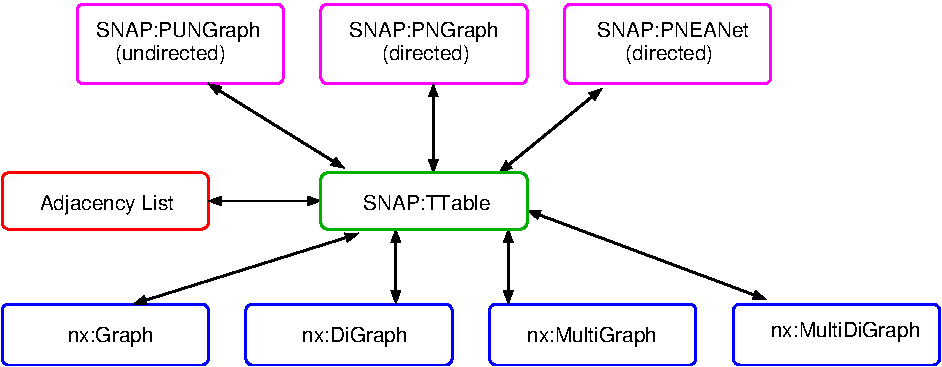
\includegraphics[scale=0.5]{figures/star_trans.pdf}
\end{center}

}

\headerbox{Acknowledgments}
          {name=Ack,column=3,row=2,below=tasks}{
{\footnotesize
This work was supported by NSF
Grants ...
}
}

\headerbox{Contact Person}
          {name=Contact,column=3,row=3,below=Ack}{
{\footnotesize
{Chris J. Kuhlman~ (\textcolor{green}{\textbf{\texttt{cjk8gx@virginia.edu}}})}
}}

\end{poster}



\end{document}
